





\documentclass[12pt,a4paper]{article}
%\usepackage[top=0.85in,left=2.75in,footskip=0.75in]{geometry}
\usepackage[english]{babel}
\usepackage[utf8x]{inputenc}
\usepackage[T1]{fontenc}
\usepackage[a4paper]{geometry}
\geometry{a4paper, top=1in, bottom=2in}
\usepackage{amsmath}
\usepackage{amssymb}
\usepackage{graphicx}
\usepackage[colorlinks=true, allcolors=blue]{hyperref}
\usepackage{epsfig,amsfonts}
\usepackage{natbib}
\usepackage{authblk}
\usepackage{subfig}
\usepackage{setspace}
\usepackage{hypcap}
\usepackage{lineno} %can do [right] to shift location of #s
%From: https://www.overleaf.com/learn/how-to/Cross_referencing_with_the_xr_package_in_Overleaf
\usepackage{xr}
\makeatletter
\newcommand*{\addFileDependency}[1]{% argument=file name and extension
  \typeout{(#1)}
  \@addtofilelist{#1}
  \IfFileExists{#1}{}{\typeout{No file #1.}}
}
\makeatother
\newcommand*{\myexternaldocument}[1]{%
    \externaldocument{#1}%
    \addFileDependency{#1.tex}%
    \addFileDependency{#1.aux}%
}
\myexternaldocument{Supplementary}

%From Lorin
\usepackage{latexsym}
\usepackage{bm}
\usepackage{bbm}

\def\eq#1{(\ref{#1})}
\def\pdf{p.d.f.\ } \def\cdf{c.d.f.\ }
\def\pdfs{p.d.f.s} \def\cdfs{c.d.f.s}
\def\mgf{m.g.f.\ } \def\mgfs{m.g.f.s\ }
\def\ci{\perp   \perp}  % conditional independence symbol
\def\beginmat{ \left( \begin{array} }
\def\endmat{ \end{array} \right) }
\def\diag{{\rm diag}}
\def\log{{\rm log}}
\def\tr{{\rm tr}}
\def\cond{\, | \,}
\newcommand*\diff{\mathop{}\!\mathrm{d}}
%\newcolumntype{P}[1]{>{\centering\arraybackslash}p{#1}}

\def\dsum{\displaystyle\sum}
\def\dint{\displaystyle\int}
%\def\dfrac{\displaystyle\frac}
\def\dsup{\displaystyle\sup}
\def\dinf{\displaystyle\inf}
\def\dmin{\displaystyle\min}
\def\dlim{\displaystyle\lim}

\newcommand{\me}{\mathrm{e}}
\newcommand{\supp}{\operatorname{supp}}
\newcommand{\abs}[1]{\left|#1\right|}
\newcommand{\comment}[1]{{\em #1}}
\newcommand{\ba}{\mathbf{a}}
\newcommand{\bb}{\mathbf{b}}
\newcommand{\bc}{\mathbf{c}}
\newcommand{\be}{\mathbf{e}}
\newcommand{\bg}{\mathbf{g}}
\newcommand{\bl}{\mathbf{l}}
\newcommand{\bs}{\mathbf{s}}
\newcommand{\bt}{\mathbf{t}}
\newcommand{\bq}{\mathbf{q}}
\newcommand{\bk}{\mathbf{k}}
\newcommand{\bv}{\mathbf{v}}
\newcommand{\bx}{\mathbf{x}}
\newcommand{\by}{\mathbf{y}}
\newcommand{\bz}{\mathbf{z}}
\newcommand{\bh}{\mathbf{h}}
\newcommand{\bu}{\mathbf{u}}
\newcommand{\bw}{\mathbf{w}}
\newcommand{\w}{\mathbf{w}}
%\newcommand{\bm}{\mathbf{m}}
\newcommand{\bp}{\mathbf{p}}
\newcommand{\bK}{\mathbf{K}}
\newcommand{\bV}{\mathbf{V}}
\newcommand{\bA}{\mathbf{A}}
\newcommand{\bB}{\mathbf{B}}
\newcommand{\bC}{\mathbf{C}}
\newcommand{\bX}{\mathbf{X}}
\newcommand{\bY}{\mathbf{Y}}
\newcommand{\bE}{\mathbf{E}}
\newcommand{\bG}{\mathbf{G}}
\newcommand{\bH}{\mathbf{H}}
\newcommand{\bP}{\mathbf{P}}
\newcommand{\bQ}{\mathbf{Q}}
\newcommand{\bR}{\mathbf{R}}
\newcommand{\bW}{\mathbf{W}}
\newcommand{\bM}{\mathbf{M}}
\newcommand{\bU}{\mathbf{U}}
\newcommand{\bZ}{\mathbf{Z}}
\newcommand{\bD}{\mathbf{D}}
\newcommand{\bI}{\mathbf{I}}
\newcommand{\bS}{\mathbf{S}}
\newcommand{\T}{\intercal}
\newcommand{\wt}{\widetilde}
\newcommand{\wh}{\widehat}

\newcommand{\E}{\mbox{E}}
\newcommand{\V}{\mbox{V}}

\newcommand{\bbE}{\mathbb{E}}

\newcommand{\bepsilon}{\boldsymbol\epsilon}
\newcommand{\bvarepsilon}{\boldsymbol\varepsilon}
\newcommand{\bbeta}{\boldsymbol\beta}
\newcommand{\bsigma}{\boldsymbol\sigma}
\newcommand{\tbbeta}{{\tilde{\boldsymbol\beta}}}
\newcommand{\tbeta}{{\tilde{\beta}}}
\newcommand{\bgamma}{\boldsymbol\gamma}
\newcommand{\bdelta}{\boldsymbol\delta}
\newcommand{\btheta}{\boldsymbol\theta}
\newcommand{\bpi}{\boldsymbol\pi}
\newcommand{\bpsi}{\boldsymbol\psi}
\newcommand{\blambda}{\boldsymbol\lambda}
\newcommand{\bphi}{\boldsymbol\phi}
\newcommand{\brho}{\boldsymbol\rho}
\newcommand{\balpha}{\boldsymbol\alpha}
\newcommand{\bmu}{\boldsymbol\mu}
\newcommand{\bomega}{\boldsymbol\omega}
\newcommand{\btau}{\boldsymbol\tau}
\newcommand{\bDelta}{\boldsymbol\Delta}
\newcommand{\bGamma}{\boldsymbol\Gamma}
\newcommand{\bOmega}{\boldsymbol\Omega}
\newcommand{\bSigma}{\boldsymbol\Sigma}
\newcommand{\bLambda}{\boldsymbol\Lambda}
\newcommand{\bTheta}{\boldsymbol\Theta}
\newcommand{\at}[2][]{#1|_{#2}}
\newcommand{\red}[1]{\textcolor{red}{#1}}
\newcommand{\blue}[1]{\textcolor{blue}{#1}}

\title{Pathway Analysis Reveals Novel Signals For Epistasis in Complex Trait Genetic Architecture Across Multiethnic Populations}
\author[1,2]{Michael C. Turchin}
\author[1,3]{Gregory Darnell}
\author[1,4,5,*]{Lorin Crawford}
\author[1,2,*,$\dag$]{Sohini Ramachandran}
\affil[1]{Center for Computational Molecular Biology, Brown University}
\affil[2]{Department of Ecology and Evolutionary Biology, Brown University}
\affil[3]{Institute for Computational and Experimental Research in Mathematics, Brown University}
\affil[4]{Department of Biostatistics, Brown University}
\affil[5]{Center for Statistical Science, Brown University}
\affil[$\ast$]{indicates these authors contributed equally}
\affil[$^\dag$]{To whom correspondence should be addressed: sramachandran@brown.edu}

\begin{document}
%\setlength{\footskip}{0cm}

\maketitle

\begin{abstract}\label{InterPath-Abstract}

\end{abstract}

\linenumbers

\section{Introduction}\label{InterPath-Introduction}

\textcolor{blue}{WIP}

It is well-established that genome-wide association studies (GWAS) are a powerful tool for identifying statistical associations between genetic variation and complex traits, and indeed have identified over XX,XXX statistically significant such associations in humans alone (citations). However, it is also becoming well-established in more recent years that GWAS and GWAS-related research directions have been incredibly focused on populations of European ancestry. In a survey of published GWAS from 2009, it was found that only 4\% of the 1.7 million individuals studied were of non-European ancestry \citep{Need2009}. Since then, other surveys suggest this percentage was on the rise until potentially plateauing around XX\% \citep{Popejoy2016,Martin2019}.

%(maybe actually keep these two paragraphs separate now? have four in total potentially?)

2009 researches were drawing attention to this skew in human ancestry attention was being brought to the imbalance of 
In a survey of published GWAS from 2009, it was found that only 4\% of the 1.7 million individuals studied were of non-European ancestry \citep{Need2009}. This report gained some brief attention, but an initial increase in the representation of non-European ancestries in GWAS has stagnated since 2014 \citep{Popejoy2016,Martin2019}; 

This is in spite of the numerous ways incorporating non-European ancestries benefit genomic analyses. In GWAS and eQTL studies, investigating more diverse sets of human ancestries can lead to more accurate effect size estimates and more novel association discoveries (page and other papers?). And lastly, having more diverse and representative reference panels can improve the performance of imputation broadly for all human ancestries (ref).  not properly accounting for population structure In  has lead to more accurate effect size estimates and larger numbers of novel loci in both GWAS and eQTL studies, as well as more precise prediction in polygenic risk scores (PRSs) \citep{Dumitrescu2011,Carlson2013,Kuchenbaecker2019,Wojcik2019}. Additionally, having more diverse datasets may allow us to better identify latent population structure, an ongoing 

The question then is why this dataset representation problem still remains so unchanged, if not beginning to worsen again. Structural issues, such as biases in funding allocations and resource availability, are certainly a major contributor. Another contributor may be a continued under appreciation of what investigating non-European populations can contribute to genomic analyses. Here, we want to show once again the profound, if not essential, benefit non-European populations provide in terms of novel insight into human complex trait genetic architecture.

As previously mentioned, since non-European populations have already provided novel insights into frameworks for conducting GWAS and PRSs, we became interested in whether non-European populations could provide similar novel insights into another genomic analysis framework, detecting genetic epistasis. Epistasis is a well-established phenomenon in a number of model organisms (citations), and has been suggested as a major component of both complex trait genetic architecture and evolution (citations). However, there remains skepticism on the extent epistasis has played a role in human populations (citations). Recent methodological advances and work has shown increasing evidence for epistasis in humans, but most epistasis work in trait genetic architecture has almost exclusively been conducted in European populations. It is unclear what novel differences or insight non-European populations might provide in epistasis, especially in light of the building evidence that additive architecture varies across human populations as well (citations).

In this study we analyzed epistasis in height and body mass index (BMI) at multiple genomic levels across six different human ancestry subsets present in the UK BioBank (UKB) \citep{Sudlow2015} dataset. We present a new methodological framework for analyzing marginal epistasis on the pathway level, and find that an African ancestry UKB subset produces many more significant epistatic pathways than any other UKB ancestry subset (XX of XX total significant pathways). We find pathways related to cellular signaling and the immune system are often represented among our significant hits, and evidence that the proteasome may be particularly enriched for epistatic interactions. We find that BMI on average produces stronger signals of pathway-level marginal epistasis than height, in line with previous results indicating BMI containing higher rates of epistatic heritability than height (citations). And lastly we find that differences between ancestries are unlikely to be due to large, broadscale patterns of genetic variation.    





Epistasis, despite being a well-established component of complex trait architecture in multiple model organisms (citations), is still regarded cautiously in human genetics (citations). Recent work has begun to show increased evidence of epistasis playing a role in human trait architecture, but still most of this research has been conducted primarily in datasets of European ancestry.


lead to more appropriate estimates of GWAS effect sizes (citations), the discovery of more novel causal loci (citations), and more accurate predictions of polygenic risk scores (citations).   

negatively impacts findings, including misestimation of  recent multiethnic investigations have discovered, including  











Genome-wide association studies (GWAS) have identified over \textcolor{red}{24,000} significant associations between individual genotypes and complex human traits \citep{Buniello2019}. However, the vast majority of these associations were identified in datasets of primarily European ancestry. In a survey of published GWAS from 2009, it was found that only 4\% of the 1.7 million individuals studied were of non-European ancestry \citep{Need2009}. This report gained some brief attention, but an initial increase in the representation of non-European ancestries in GWAS has stagnated since 2014 \citep{Popejoy2016,Martin2019}; this lack of representation is even more disconcerting given the ongoing explosion of available human genomic data. 

It was largely hoped during the GWAS era that human genetic architecture would be consistent across human ancestries, for instance that causal loci and association effect sizes would remain the same among different human populations \citep{Need2009,Pulit2010,Bustamante2011,Bien2019}. However, recent work has begun to directly interrogate this assumption, and the initial findings are indeed showing that genetic architecture is often not the same between human ancestries; studies have shown that not only are association effect size estimates different between ancestries, but at times even causal loci appear to differ as well \citep{Dumitrescu2011,Carlson2013,Kuchenbaecker2019,Wojcik2019}. Additionally, polygenic risk score studies, where published effect size estimates are used to predict phenotypes in other populations, are showing that applying European-based estimates to non-European populations consistently produce erratic and nonsensical results \citep{Martin2017,Duncan2019,Kerminen2019,Rosenberg2019}.

It is clear both that non-European populations are incredibly underrepresented in modern GWAS studies and that European populations cannot act as accurate proxies for the rest of the world. Therefore there is an massive need for work that explores the many aspects of complex trait genetic architecture in non-European populations. To help address these needs, we focus here on investigating the importance of epistasis, or genetic interactions, in complex traits across multiple non-European populations. 

Epistasis, despite being a well-established component of complex trait architecture in multiple model organisms (citations), is still regarded cautiously in human genetics (citations). Recent work has begun to show increased evidence of epistasis playing a role in human trait architecture, but still most of this research has been conducted primarily in datasets of European ancestry. Therefore to address this unexplored area of research, we investigated epistasis at multiple genomic scales across multiple European and non-European populations. We extracted both European and non-European subsets from the UK BioBank (UKB) \citep{Sudlow2015} and identified evidence for epistasis on the SNP-level, pathway-level, and the genome-wide level. We identify that evidence for epistasis varies across human ancestries, and that African populations often have greater evidence for epistasis. We present a novel framework for combining epistasis and pathway analysis and identify pathways that have both population-specific evidence for epistasis as well as pathways that appear to have significant levels of epistasis worldwide. And lastly, we show beginning evidence that one of the driving factors for the higher levels of epistasis apparent in non-European populations may be greater levels of population-wide genetic diversity.





\section{\textcolor{red}{Results (please read all of Results, thanks!)}}\label{InterPath-Results}

\subsection{Single-SNP Methods Provide Limited Evidence For Epistasis}\label{InterPath-Results-SNPEpistasis}

To begin investigating epistasis in non-European ancestries, we first extracted multiple non-European population subsets from the UK BioBank (UKB) dataset, including individuals of African, Caribbean, Chinese, Indian, and Pakistani self-identified ancestry (Supplementary Figure \ref{InterPath-Supp-Figure-UKB-Subsets-PCAPlot} and Table \ref{InterPath-Supp-Table-UKBPopStats}). For comparative purposes, we also extracted a British subset; but to make it on a matched scale as the non-European subset sample sizes, we used a random subsample of 4,000 British individuals. Across all these population subsets, we conducted typical quality control (QC) procedures (see Materials and Methods) and focused our analyses on the complex traits of height and body mass index (BMI). 

To analyze epistasis on the single variant level, we take two different approaches. First, we ran the canonical model of pairwise SNP interactions implemented by PLINK (see Materials and Methods). This approach exhaustively searches through every pairwise set of SNPs and tests whether there is a significantly non-zero interaction effect size. Running this method on each of our population subsets we find that no pairs of SNPs produce a genome-wide significant interaction (Supplementary Figure \ref{InterPath-Supp-Figure-PLINK-HeightBMI-AllPops}). Here we define `genome-wide significant' as having an interaction $p$-value $<= 5\times10^{-13}$, which is the approximate Bonferroni-corrected $p$-value threshold given the over $1\times10^{11}$ number of tests that were conducted. This lack of significant results may not be surprising given such a heavy multiple-testing burden. Alternatively, we can forgo such a stringent criteria and instead look at SNPs that are marginally significant ($p$-value $<= 1\times10^{-4}$); since this produces many possible interactions per SNP, we can also instead look at the \textbf{proportion} of marginally significant interactions per SNP as a more appropriate metric.  

Looking at this new framework, we do start to see different patterns between our ancestry subsets (Supplementary Figure \ref{InterPath-Supp-Figure-PLINK-Proportions-HeightBMI}). We find that different areas of the genome are producing SNPs with large proportions of marginally significant interactions across our different subsets (Supplementary Table \ref{InterPath-Supp-Table-PLINK-Proportions-TopSNPs-a}), as well as different baseline levels of marginally significant interactions between ancestry subsets as well (such as the Chinese and Pakistani subsets having the largest baseline interactions in height). However, we once again do not have many individual SNPs that particularly stand out. 

The second approach we took to investigate single-SNP epistasis was to implemented MAPIT \citep{Crawford2017}, a method which specifically tests for the presence of \textit{marginal epistasis} (see Materials and Methods). In brief, the marginal epistasis of a single SNP can be thought of as the summation of \textbf{all} epistatic interactions that SNP has with the rest of the genome. Evidence for marginal epistasis does not immediately identify \textbf{which} loci elsewhere in the genome the SNP of interest is interacting with, but in exchange for this generalization the approach turns a highly burdensome multiple-testing setup into a much more tractable variance component model.

Running MAPIT on our population subsets for both height and BMI, we find that there are no SNPs with genome-wide significant signals for marginal epistasis ($p$-value $<= 5\times10^{-8}$; Supplementary Figure \ref{InterPath-Supp-Figure-MAPIT-HeightBMI}). We do also see once again however the top SNPs occurring in different regions of the genome between our different population subsets (Supplementary Table \ref{InterPath-Supp-Table-MAPIT-TopSNPs-a}). But it is unclear if these are results reflecting true biology or simply noise due to a lack of power. Going along with the theme of relaxing our significance threshold criteria to help identify patterns, we compared our MAPIT results against our PLINK results. Specifically, we compared each SNP's MAPIT -$\log_{10}$ $p$-value against its proportion of marginal significant PLINK interactions, and indeed we see more potential evidence for signals of epistasis (Figure \ref{InterPath-Main-Figure-PLINKvsMAPIT-HeightBMI-African} \& Supplementary Figure \ref{InterPath-Supp-Figure-MAPITvsPLINK-HeightBMI-AllPops-a}). Looking at height and BMI in the African subset for example, we see that for some SNPs that have marginally significant MAPIT $p$-values, they also have greater proportions of marginally significant pairwise SNP interactions. Because these two metrics are potentially measuring the same thing but through different approaches, seeing marginal signals from both methods at the same locus is encouraging. Therefore, despite our limited power to identify single-SNP genome-wide significant interactions, there may be evidence for epistasis at lower stringency thresholds in our data.

\begin{figure}[htb]
\centering
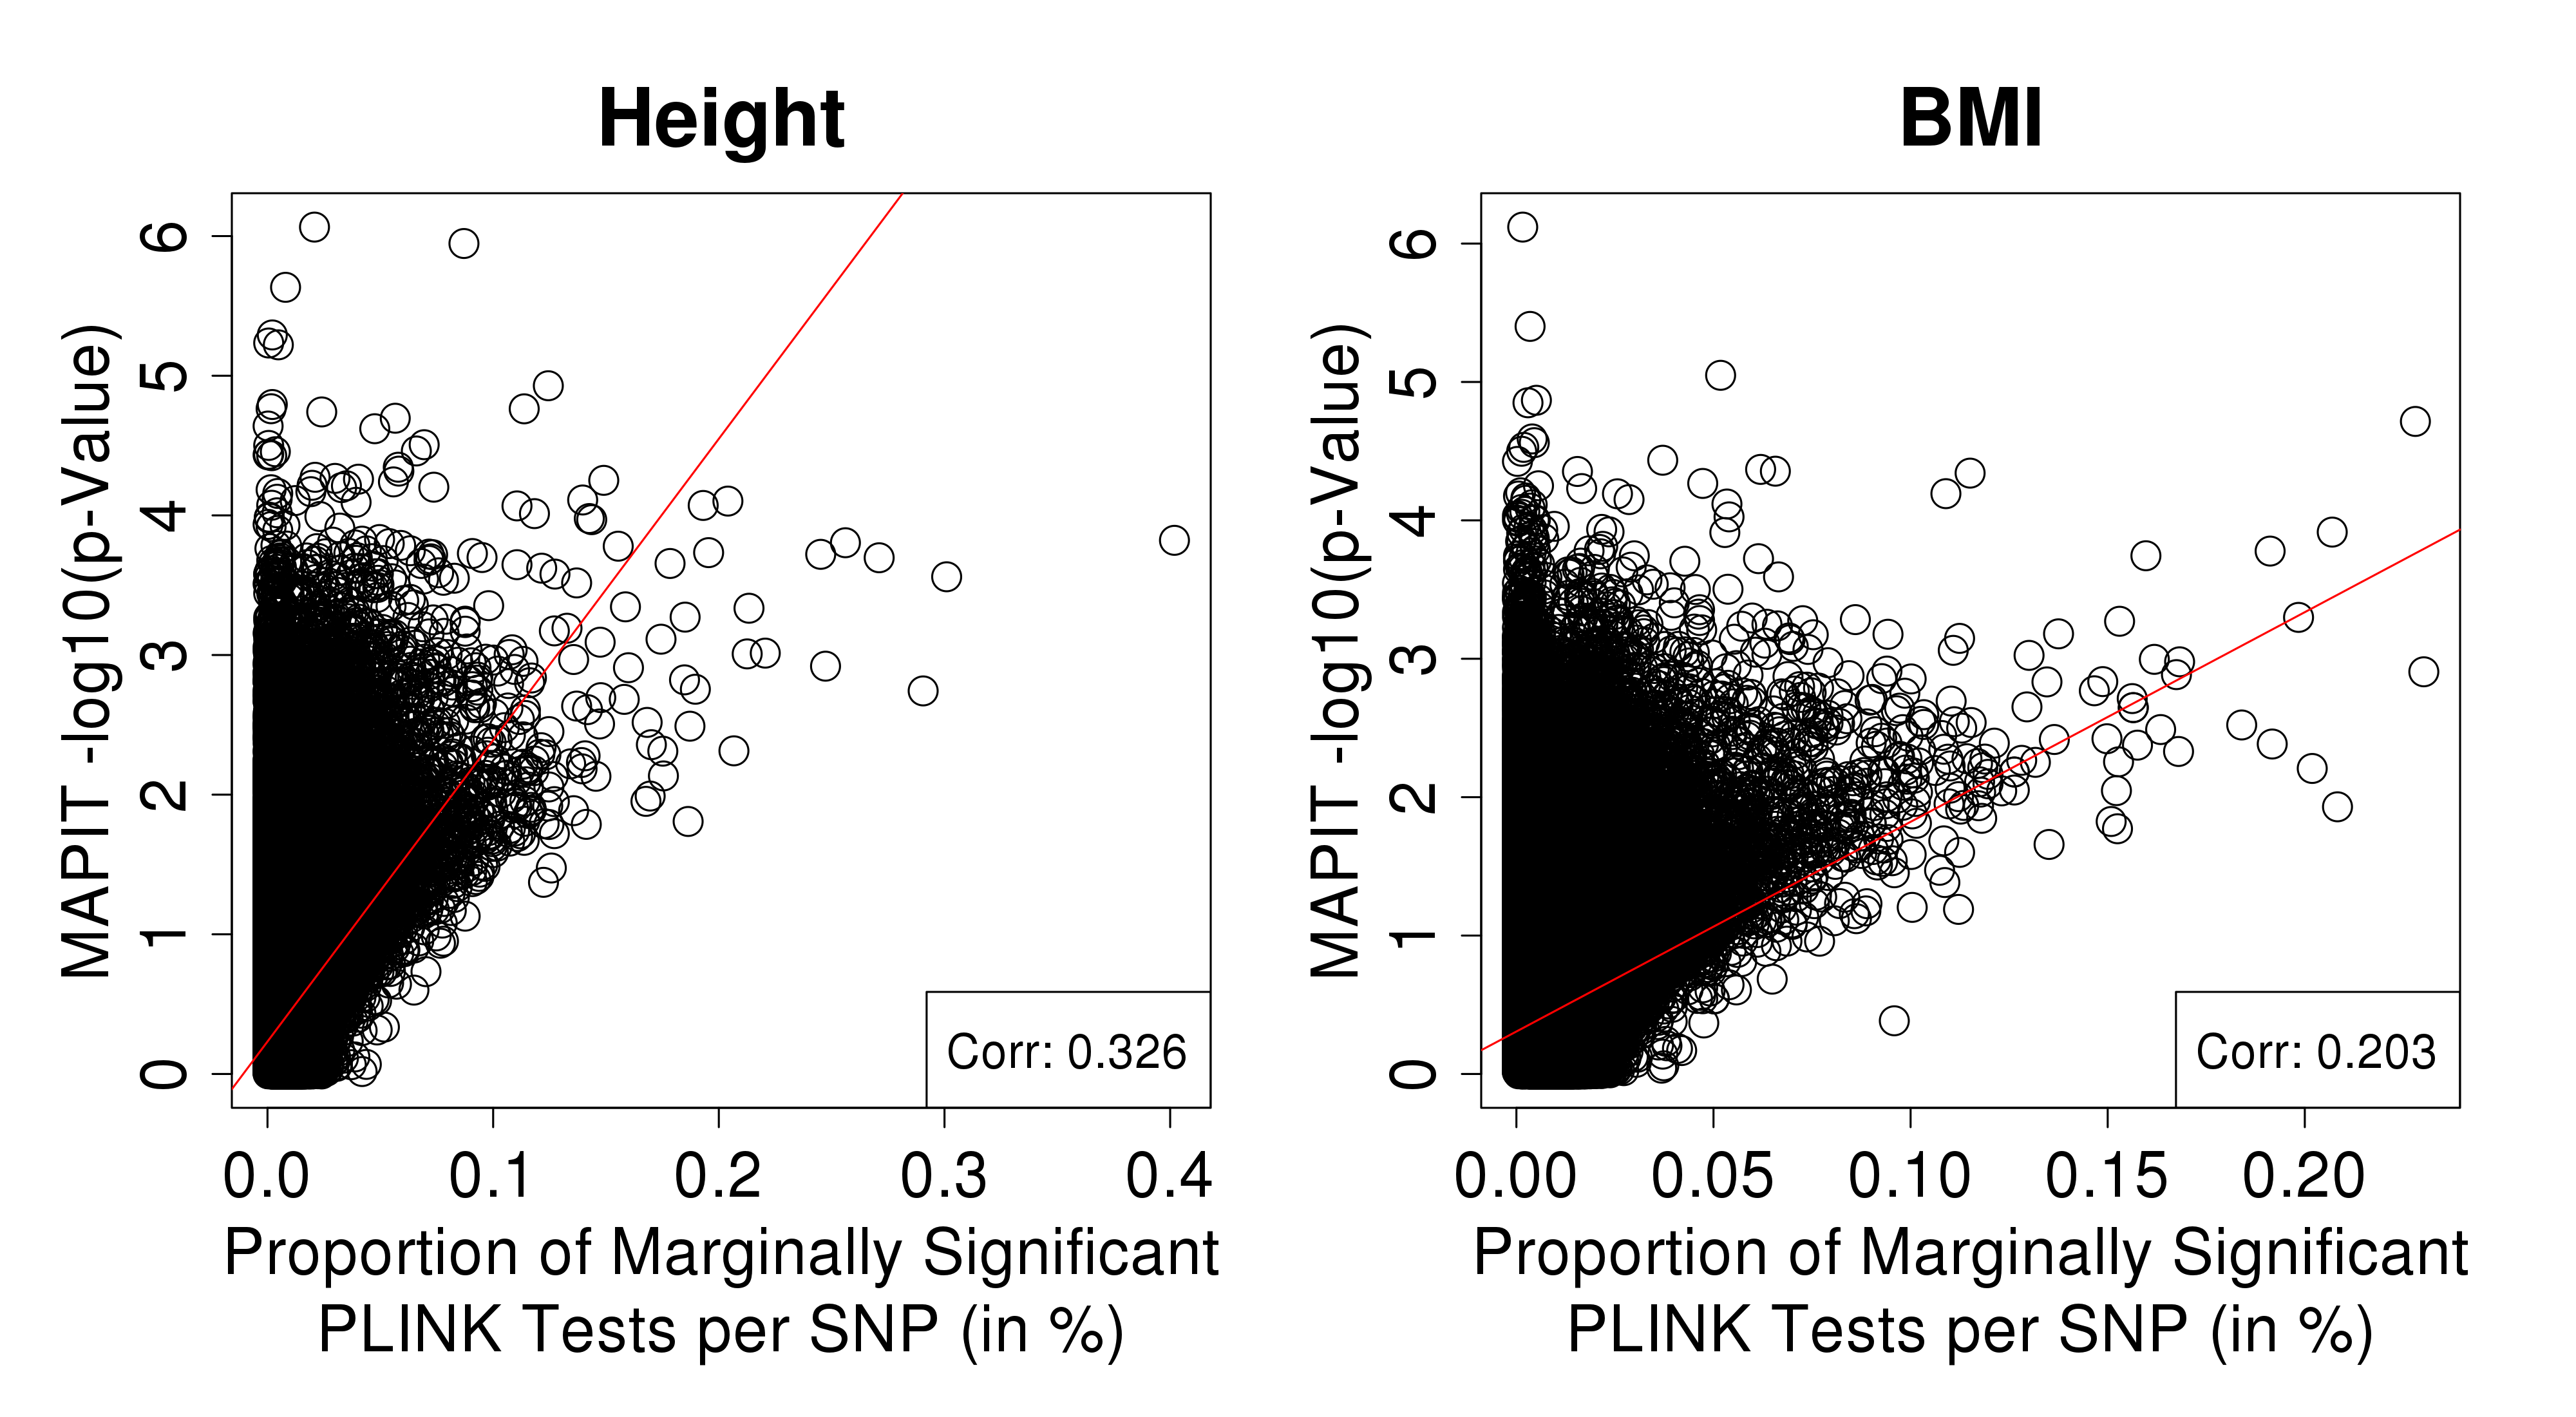
\includegraphics[scale=.45]{Images/Main/InterPath_Main_Figure_PLINKvsMAPIT_vs3_African_HeightBMI.png}
\caption[TBD]{\textbf{Comparison of single-SNP epistasis methods in African subset}. The figure shows the single-SNP PLINK results vs. MAPIT results for height and BMI in the African subset. The PLINK results are shown on the $x$-axis as the proportion of marginally significant interactions per SNP (where marginally significant is defined as $p$-value $<= 1\times10^{-4}$) and the MAPIT results are shown on the $y$-axis as the -$\log_{10}$ of the MAPIT $p$-values. The dotted red line shows the line of best fit, and the correlation between the two metrics is shown in the legend. We observe a subset of SNPs with greater marginal epistasis (higher -$\log_{10}$ $p$-values) beginning to correlate with having larger proportions of marginally significant SNP-by-SNP interactions. Seeing the same signal between two different approaches suggests there may be evidence for epistasis on the single-SNP level, albeit weak. For the same plots across all UKB subsets, see Supplementary Figure \ref{InterPath-Supp-Figure-MAPITvsPLINK-HeightBMI-AllPops}.}
\label{InterPath-Main-Figure-PLINKvsMAPIT-HeightBMI-African}
\end{figure}

There remains the issue though of our limited sample sizes and datasets. As previously discussed, there are ongoing efforts to increase the number of non-European individuals publicly available for complex trait analysis \citep{Matise2011,Kowalski2019}, but these numbers still currently pale in comparison to what is available for European individuals \textcolor{red}{(I'm assuming we'll be bringing this up in the Introduction, so I'm anticipating calling back to that here in some manner)}. Therefore, we need to identify ways to continue making better use out of the datasets we currently have. The approaches we have used thus far here have revolved around testing single variants. However, it has long been appreciated in other methodological areas, such as additive work, that aggregating evidence for association across multiple variants can increase power to detect significant signals \citep{}. Therefore, we decided to explore whether taking a similar approach towards epistatic analyses would lead to an increase in power as well. And the marginal epistasis framework provides a natural model for just such an extension. 

\subsection{Many Pathways Identified As Genome-Wide Significant for Marginal Epistatic Interactions in the African Subset}\label{InterPath-Results-PathwayEpistasis}

Therefore we created a new method by expanding the previous MAPIT framework into a new model that goes from identifying single-SNP marginal epistasis to identifying multiple-SNP marginal epistasis; we call this approach MAPIT-R, for \underline{MA}rginal e\underline{PI}stasis \underline{T}est for \underline{R}egions. For a full description of this new model please see Materials and Methods, but in brief the main change we make is to go from a single SNP of interest \textbf{k} to a collection of SNPs of interest \textbf{R}. This in turns leads us to incorporate a new random effect  \textbf{Q} that represents the epistatic interactions between all the SNPs in \textbf{R} with all the remaining variants (SNPs not in \textbf{R}) across the genome. Using the same MQS \citep{Zhou2017} setup as MAPIT did, we then test whether the variance component associated with \textbf{Q}, $\phi$ is significantly different from zero. If $\phi$ is significantly different from zero, it indicates that there is detectable marginal epistatic interactions between our group of SNPs \textbf{R} and the rest of the genome.

Since this is a generalizable approach that allows for any set of SNPs \textbf{R} to be tested, we decided to begin by using known biological pathways. Specifically, we utilized the KEGG and REACTOME pathway datasets from the MSigDB \citep{Liberzon2011}; we chose these pathways due to their coverage of a wide range of biological processes as well as their wide range of pathway gene sizes. This would not only potentially allow us to investigate what the effect of different \textbf{R} sizes may be on our approach, but also provide biological starting points for any putative results. Additionally, this would be the first time marginal epistasis has been investigated on the pathway scale in human populations.

Running MAPIT-R on our UKB subsets across height and BMI, we find 245 pathways that are genome-wide significant for containing marginal epistatic interactions with the rest of the genome (Figure \ref{InterPath-Main-Figure-Barplots-KEGG}, Supplementary Figure \ref{InterPath-Supp-Figure-Barplots-REACTOME}, and Supplementary Tables \ref{InterPath-Supp-Table-TopPathways-KEGG-Height-a}\textcolor{blue}{-d}; $p$-value significance thresholds were determined using Bonferroni multiple testing correction based on the number of pathways tested per analysis). We find similar numbers of significant pathways between the KEGG and REACTOME databases, though KEGG contains more significant hits (130 vs. 115). And in both databases, we find that BMI contains more significant pathways than height (155 vs. 90). Interestingly, the vast majority of our significant pathways are identified in the African subset (165/245). This abundance in the African subset is found in each pathway database as well as in each phenotype.   

Looking at which specific pathways are significant in the African subset, we see multiple themes across each of the database and phenotype combinations (Supplementary Tables \ref{InterPath-Supp-Table-TopPathways-KEGG-BMI-a}\textcolor{blue}{-d}). In KEGG height, we find multiple pathways representing cellular signaling (e.g. KEGG\_CHEMOKINE\_SIGNALING\_PATHWAY, KEGG\_CYTOKINE\_CYTOKINE\_RECEPTOR\_INTERACTION, and \\ KEGG\_WNT\_SIGNALING\_PATHWAY), immune systems (e.g. \\ KEGG\_AUTOIMMUNE\_THYROID\_DISEASE, KEGG\_ALLOGRAFT\_REJECTION, and KEGG\_ANTIGEN\_PROCESSING\_AND\_PRESENTATION), and heart conditions (e.g. KEGG\_DILATED\_CARDIOMYOPATHY and \\ KEGG\_VIRAL\_MYOCARDITIS). In KEGG BMI, we find similar themes, as well as multiple pathways that involve metabolism (e.g. KEGG\_PURINE\_METABOLISM, KEGG\_BETA\_ALANINE\_METABOLISM, and \\ KEGG\_ETHER\_LIPID\_METABOLISM). REACTOME pathways show similar themes as well in both phenotypes.

\begin{figure}[htb]
\centering
\hspace*{-.9cm}
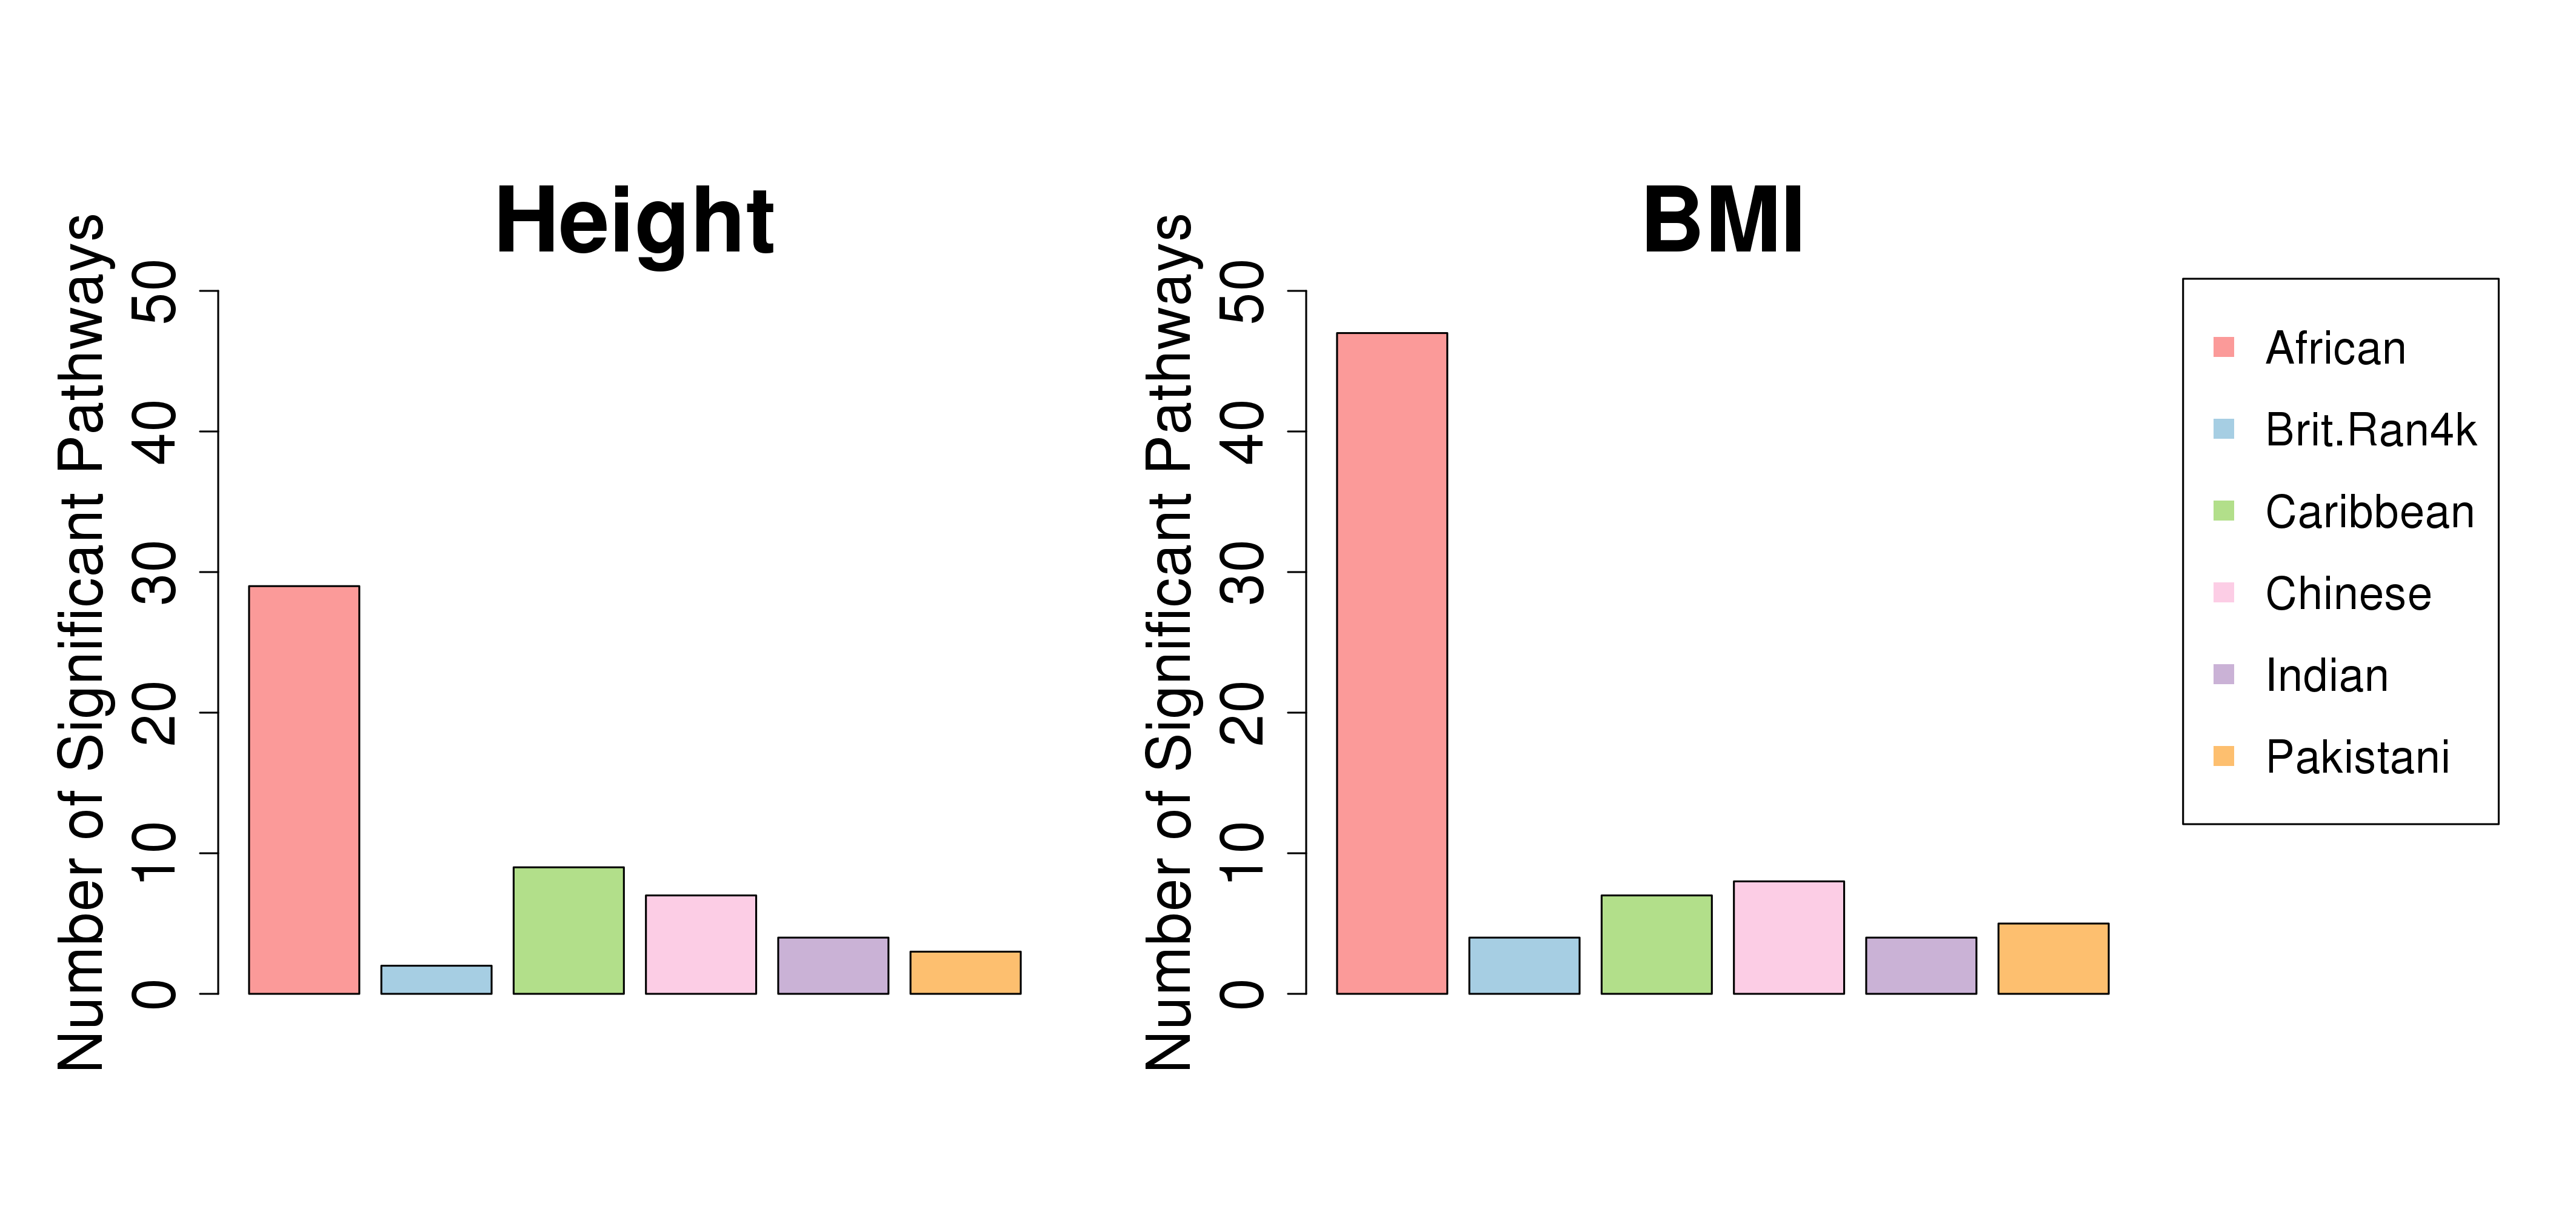
\includegraphics[scale=.45]{Images/Main/InterPath_Main_Figure_Barplots_KEGG_vs2.png}
\caption[TBD]{\textbf{Number of KEGG pathways that have significant marginal epistasis, per subset}. The figure shows the number of genome-wide significant pathways found from running MAPIT-R for height and BMI in the KEGG database on each of our UKB subsets. Results from the REACTOME database in height and BMI can be found in Supplementary Figure \ref{InterPath-Supp-Figure-Barplots-REACTOME}. Genome-wide significance was determined by using Bonferroni-corrected $p$-value thresholds based on the number of pathways tested in each phenotype, subset, and pathway database combination. As shown in these results, we find across all phenotype and database combinations that the African subset has the largest numbers of significant pathways. For lists of the specific significant pathways per subset, phenotype, and database combination, see Supplementary Tables \ref{InterPath-Supp-Table-TopPathways-KEGG-Height-a}\textcolor{blue}{-d}.}
\label{InterPath-Main-Figure-Barplots-KEGG}
\end{figure}

This abundance of signal in the African subset stands out since the African subset is neither our subset with the largest sample size or our subset with the largest number of SNPs (Supplementary Table \ref{InterPath-Supp-Table-UKBPopStats}). Therefore it is important to consider alternative reasons that might explain this result aside from it being representative of true underlying biological patterns. \textcolor{red}{One alternative explanation for this result may be an ascertainment bias from using variants based on a genotyping chip that was developed primarily using European data. Simulations that replicate such an ascertainment bias however show no evidence of this leading to an increase in power (Supplementary Figure XX). Another possible alternative explanation is that these results are products of uncorrected, residual population structure. While we do include top principal components as covariates in our analysis, we conducted additional simulations that explicitly model population structure, and we once again find no evidence that this may be affecting our results (Supplementary Figure XX). (this is what we hope to get from Greg's work).} Lastly, we also ran versions of our analysis using permuted phenotypes to broadly check if our method behaves appropriately under the null and indeed find this to be the case (Supplementary Figures \ref{InterPath-Supp-Figure-perm1-QQPlots-AllPaths} and \ref{InterPath-Supp-Figure-10perms-pValHists}); we also used these permutations to investigate our FDRs and observe rates only as high as 1.5\% across our different ancestry, phenotype, and pathway database combinations at different significance thresholds (Supplementary Table \ref{InterPath-Supp-Tables-AllPops-FDRs}).

\subsection{Beginning Examples of Ancestry-Level Differences in Epistatic Interactions}

Expanding beyond the results from our African subset, we see 80 other pathways that are significant across the other subpopulations. Perhaps unsurprisingly given the abundance of results from the African subset, many of these other results overlap with the set of significant pathways from the African subset (Figure \ref{InterPath-Main-Figure-Heatplots-KEGG} \& Supplementary Figure \ref{InterPath-Supp-Figure-Heatplots-REACTOME}). For example, in the KEGG Height results the Caribbean subset overlaps with the African subset for 6 of its 7 pathways, and the Chinese subset overlaps with the African subset for 7 of its 8 pathways; interestingly, however, there is no overlap between the Chinese and Caribbean subsets. 

\begin{figure}[htb]
\centering
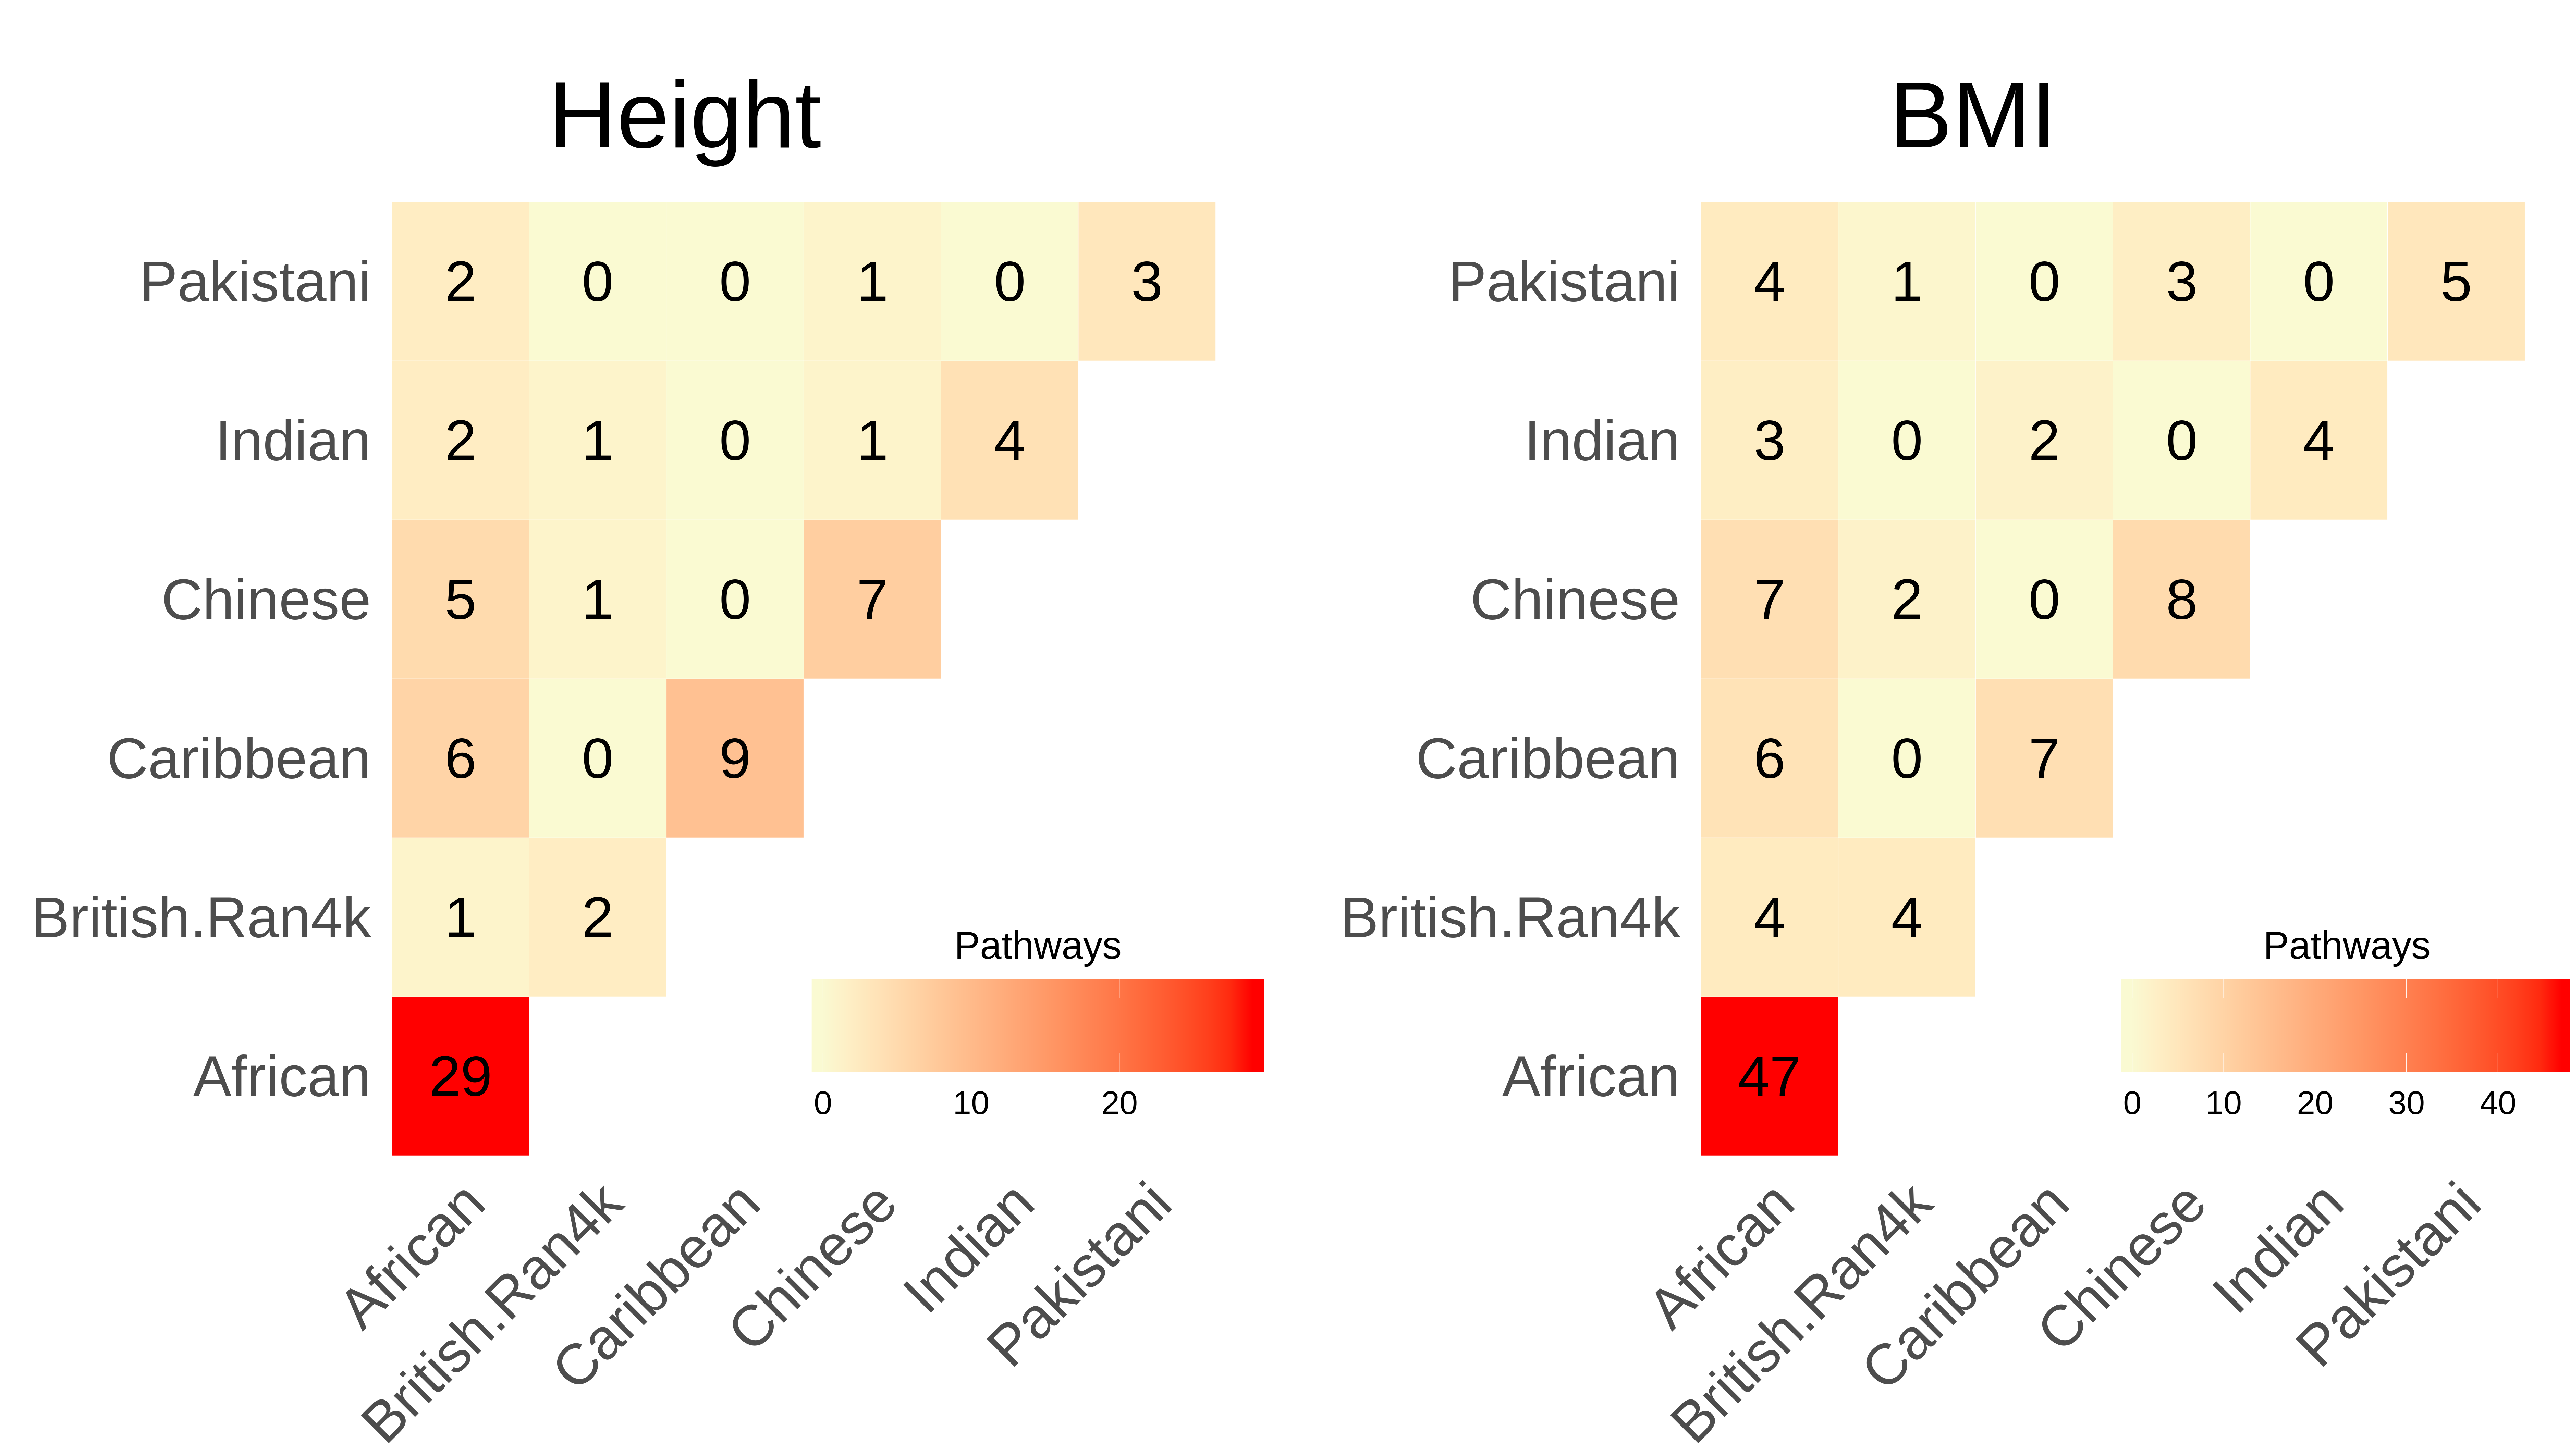
\includegraphics[scale=.225]{Images/Main/InterPath_Main_Figure_Heatplots_KEGG_vs2.png}
\caption[TBD]{\textbf{Overlap of MAPIT-R significant KEGG pathways between UKB subsets}. The heatplots show the numbers of genome-wide significant MAPIT-R pathways that overlap between each UKB subset for height and BMI in the KEGG database. Results for both phenotypes in the REACTOME database can be seen in Supplementary Figure \ref{InterPath-Supp-Figure-Heatplots-REACTOME}. The diagonal shows the total number of genome-wide significant pathways per population subset. We observe that most subsets often have overlap with the African subset but rarely do so with the remaining non-African subsets.}
\label{InterPath-Main-Figure-Heatplots-KEGG}
\end{figure}

Looking into the specific pathways in each of these overlaps, we find pathways moreso related to the cellular signaling and heart condition patterns from before in the overlap between the African and Caribbean subsets; additionally these overlaps appear to be driven by multiple kinases (eg MAPK1, ROCK1, PRKCB, PAK1) and calcium channel proteins (eg CACNA1S, CACNA1D) (Supplementary Tables \ref{InterPath-Supp-Tables-MAPITR-TopPathway-Overlap} \& \ref{InterPath-Supp-Tables-MAPITR-TopPathway-GeneCounts-Overlap}). The overlap between the African and Chinese subsets however moreso contain pathways related to the immune system and appear to be driven primarily by multiple HLA loci (eg HLA-DRA, HLA-DRB1, HLA-A, HLA-B) (Supplementary Tables \ref{InterPath-Supp-Tables-MAPITR-TopPathway-Overlap} \& \ref{InterPath-Supp-Tables-MAPITR-TopPathway-GeneCounts-Overlap}). These differences between ancestries may reflect heterogeneous power to detect epistatic signals. It is interesting to see the continual overlap between non-African subsets and the African subset, but less so between the non-African subsets. One possibility we may be witnessing is that pathways with the largest signals for marginal epistasis may be widely important biologically, hence seeing themes such as cellular signaling and the immune system. More population-specific signals may require greater sample sizes to identify. 

\subsection{BMI Contains Stronger Signals than Height for Marginal Epistatic Interactions}

Focusing once again on the African results, we observe in both the KEGG and REACTOME databases more significant pathways in BMI than Height. While there is a strong correlation between the MAPIT-R -$\log_{10}$ $p$-values of these two phenotypes (.851 in KEGG and .858 in REACTOME), we consistently see more significant signals in BMI (Figure \ref{InterPath-Main-Figure-MAPITR-PhenoComps-African}). This may not be a surprising result since pedigree-based heritability estimates have suggested narrow-sense heritability is around .8 in height and between .4 and .6 in BMI \citep{Elks2012,Visscher2012}; this would suggest that non-additive effects may play a greater role in BMI than height, which aligns with our results here. 

\begin{figure}[htb]
\centering
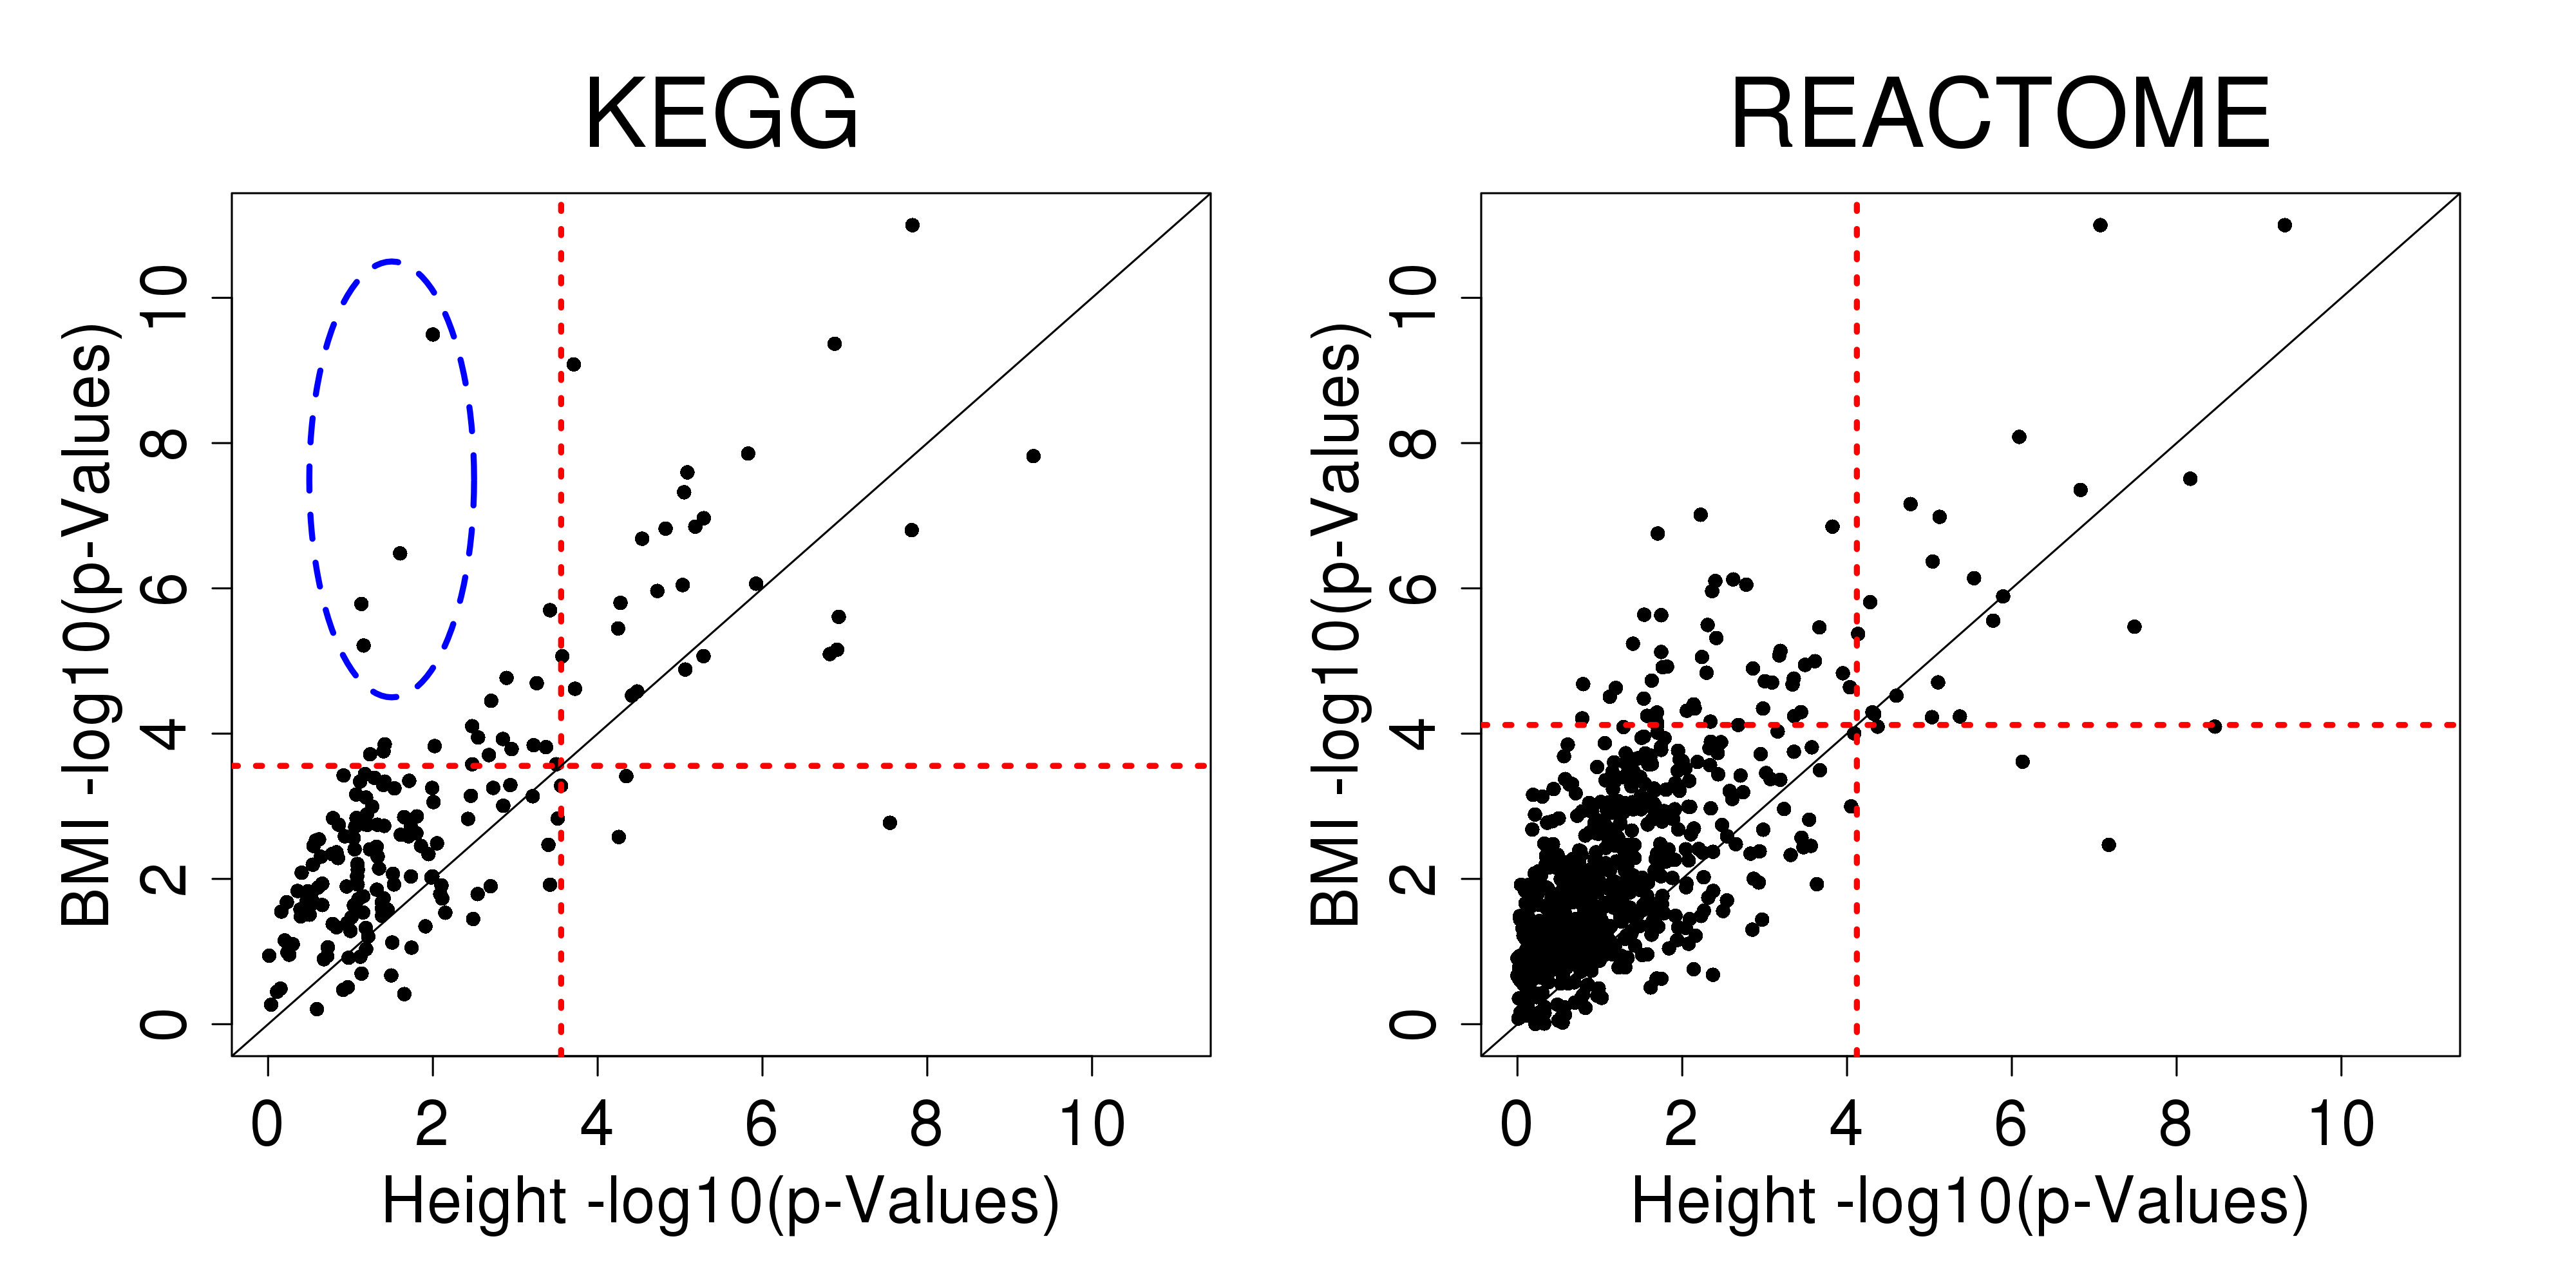
\includegraphics[scale=.45]{Images/Main/InterPath_Main_Figure_MAPITR_PhenoComps_African_vs3.png}
\caption[TBD]{\textbf{Comparison of MAPIT-R results between height and BMI in the African subset}. The figure shows MAPIT-R height results plotted against MAPIT-R BMI results for all pathways from the KEGG and REACTOME databases in the African subset. The $x$-axis is the MAPIT-R height -$\log_{10}$ $p$-value and the $y$-axis is the MAPIT-R BMI -$\log_{10}$ $p$-value. The dotted red lines are the Bonferroni-corrected $p$-value thresholds for genome-wide significance in each pathway and phenotype combination. The blue ellipse in the KEGG results highlight four pathways that appear to have much more significant BMI $p$-values than height $p$-values. In general though, across both pathway databases, we see more significant $p$-values in BMI than height. For these comparisons in all the UKB subsets, see Supplementary Figure \ref{InterPath-Supp-Figure-MAPITR-PhenoComps-AllPops}.}
\label{InterPath-Main-Figure-MAPITR-PhenoComps-African}
\end{figure}

Looking specifically at pathways that diverge in significance between height and BMI, we find one cluster of pathways in the KEGG results that separate out as particularly more significant in BMI than height. The four pathways circled in Figure \ref{InterPath-Main-Figure-MAPITR-PhenoComps-African}, sorted by decreasing -$\log_{10}$ $p$-value, are KEGG\_SMALL\_CELL\_LUNG\_CANCER, KEGG\_ERBB\_SIGNALING\_PATHWAY, KEGG\_NON\_SMALL\_CELL\_LUNG\_CANCER, and KEGG\_T\_CELL\_RECEPTOR\_SIGNALING\_PATHWAY. We once again see this theme of signaling pathways, but now also a trend of oncogenic pathways. Looking at the genes driving these pathways (Supplementary Table \ref{InterPath-Supp-Table-MAPITR-PhenoComps-African-GeneCounts}), we find two sets of gene families that appear in all four pathways: phosphatidylinositol 3-kinases (PIKs) and the AKT serine/threonine-protein kinases. One gene that stands out from this group is AKT2, a locus that has been associated with multiple monogenic disorders of glucose metabolism, including severe insulin resistance and diabetes, and severe fasting hypoinsulinemic hypoglycemia \citep{George2004,Manning2017,Latva-Rasku2018}. This gene might be a strong candidate then for having epistatic interactions more relevant to BMI than height, possibly explaining this cluster of pathways.       

\subsection{The Proteasome is Enriched for Marginal Epistatic Interactions}

To look deeper into our African subset results, we were interested in whether any genes were significantly enriched across our top pathways. Finding genes that are significantly enriched could potentially provide greater insight into what biology is underlying our pathway results, or even identify new biological patterns all together. To accomplish this we began with the canonical approach of using the hypergeometric test for enrichment; here, we will compare the number of times a gene appears among our significant pathways against the number of times that gene appears in the full distribution of pathways in either the KEGG or REACTOME databases. 

Supplementary Tables \ref{InterPath-Supp-Tables-AllPops-TopGeneCounts-KEGG-Height-a}\textcolor{blue}{-d} shows the various genes present across our significant pathways at different levels of counts, and Supplementary Figure \ref{InterPath-Supp-Figure-Hypergeometric-QQPlots-African} shows the QQ-plots of our hypergeometric enrichment results across these genes. What immediately stands out is the abundance of `significant' $p$-values we find. For example, using the conservative Bonferroni cutoff of $2.082\times10^{-5}$ (.05 / 2401 genes), we would identify 45 genes as being significantly enriched in the REACTOME BMI analysis. However, one major assumption underlying this test is that each pathway is independent from one another, and we know this to not be the case. In fact this assumption is being violated in two ways in regards to the distribution of pathways we are analyzing. 

First, we know that many pathways overlap one another in terms of gene content, and that this particular set of relationships is not easily deconstructed. Second, we also know that the hypothesis underlying our approach is that more SNPs should be correlated to greater levels of significance, and this is indeed what we observe in the results (Supplementary Figure \ref{InterPath-Supp-Figure-pValsVsNumSNPs}); across both phenotypes in both pathway databases, we observe significant relationships between MAPIT-R -$\log_{10}$ $p$-values and the number of SNPs present in an analyzed pathway. This is encouraging in that it supports our initial intuition, but it does lead to significant pathways being more likely to have many SNPs and genes. Therefore when we observe a gene as significantly enriched, it may be possible that the locus just happens to be present in many pathways due to the nature of its function, such as being a `housekeeping' gene. In this case, the enrichment may be less a reflection of our biological interest (genes enriched for epistatic interactions) and more a reflection of the quality of the pathway databases (larger pathways have more similar gene content than smaller pathways do).

The second of these two situations is what we tried to resolve first. If we are concerned about a relationship between larger pathways and inflated hypergeometric $p$-values, then one possible approach might be to restrict the size of the pathways analyzed. Instead of looking at enrichment among all pathways, we can instead look at enrichment only among pathways that have under a certain number of SNPs. And indeed, by restricting the number of SNPs present in a pathway to 1,000 or less, we see a major drop off in the number of significant pathways remaining (29 to 2 for KEGG height, 47 to 11 for KEGG BMI, 24 to 0 for REACTOME height, and 65 to 26 for REACTOME BMI); this, by extension, also produces a large drop in the genes that are present across these pathways as well as their associated hypergeometric $p$-values (Supplementary Figure \ref{InterPath-Supp-Figure-Hypergeometric-RestrictedComps-African-BMI} and Supplementary Table \ref{InterPath-Supp-Table-Hypergeometric-RestrictedComps-African-BMI-TopExamples}). Interestingly however, we find one gene family that has had the opposite result -- multiple proteasome subunit genes (\textit{PSMA}*, \textit{PSMB}*, \textit{PSMC}*, \textit{PSMD}*, and \textit{PSME*}) now produce more significant hypergeometric $p$-values upon this restriction to pathways with smaller SNP counts (Supplementary Table \ref{InterPath-Supp-Tables-AllPops-TopGeneCount-HypergeometricTests}). 

The proteasome is one half of the ubiquitin-proteasome system (UPS), a critical process for proper protein degradation and cell homeostasis \citep{Voges1999,Livneh2016,Collins2017}. And the genes highlighted in this size-restricted analysis represent both the core (20S) and regulatory cap (19S or 11S) subunits of the 26S proteasome, the main variant found within the cytosol of mammalian cells. Looking at the size-restricted pathways these genes are present in, we see multiple pathways related to cell-cycle regulation and, once again, the immune system (Supplementary Table \ref{InterPath-Supp-Tables-AllPops-TopGeneCount-SizeRestricted-Proteasome}). This new, first, category makes sense since protein levels (and therefore their regulation and degradation) are a key component of determining when cells progress through various cycle checkpoints. Encouragingly, these pathways also contain a range of SNP sizes, including multiple pathways with less than 600 SNPs -- this suggests that the results are not simply the product of finding pathways with the next largest set of SNP sizes, which would potentially have the most power \textit{a priori}, but are instead being driven by other factors, such as the underlying biology. More work will be needed to investigate whether these particular results are unique to BMI or are representative of a broadly important protein complex for many phenotypes. But overall these results suggest the proteasome is a prime candidate as a protein complex that is significantly enriched for marginal epistatic interactions.  

%To further look into these proteasome genes, we...

\subsection{Testing the Null Model with British Replicate Subpopulations}

One important consideration of our results is that we have limited representations of the different human ancestries we are analyzing. Are the samples we are analyzing large enough to be representative of the true total populations? While it is still difficult to address that question directly for non-European populations due to the limited availability of other public datasets, we are able to ask that question for the British ancestry subsets. Specifically, we can take additional, non-overlapping random subsets of 4,000 British individuals and see if they are at least consistent in their lack of results as compared to the original random subset. Furthermore, given the data availability, we also constructed sets of larger British subsamples to investigate the impact of sample size on our results as well. In total we analyzed 5 sets of 4,000 British individuals and 5 sets of 10,000 British individuals. 

And overall we see similar results across all replicates to our original results from the first set of 4,000 British individuals. We see limited numbers of significant pathways across all replicate subset, phenotype, and database pathway combinations, as well as limited overlap of significant pathways between replicates (Supplementary Figures \ref{InterPath-Supp-Figure-BritReps-Barplots}\textcolor{blue}{-13}). We also ran analyses using permuted phenotypes, as before, and once again see proper behavior under the null and very low FDRs (Supplementary Tables \ref{InterPath-Supp-Tables-BritReps-FDRs-pt1}). While not presenting new significant pathways, these results at least suggest that the large numbers of significant pathways we observe in the African subset are less likely to be a product of simply choosing a particularly optimal set of individuals by chance.  

\subsection{Investigating the Relationship Between Within-Population Genetic Structure and Detecting Epistasis}

It is clear that the African subset produces many more significant MAPIT-R results than any other subset in our analysis; an obvious next question then is: why? It is known that on average African populations harbor greater levels of genetic variation than other global human populations. It may be possible that having greater base levels of variation across the genome may provide more power for our approach. Therefore we began to investigate whether there were any links between different population genetic measures of genetic variation within our subsets and their respective MAPIT-R results.

Our first approach to investigate this question was to look at broadscale metrics of genetic variation across our population subsets. We did this by calculating both pairwise F\textsubscript{ST} values between each subset as well as PVE estimates for each subset's top 10 local principal components (Figures \ref{InterPath-Main-Figure-Fst} \& \ref{InterPath-Main-Figure-Eigenvalues}). For pairwise F\textsubscript{ST}, we find values as large as .124, which seem to be within range of previous global sample estimates \citep{Wang2012}. We find that while the African subset does have some of the largest divergences from other populations (such as the British subsets), we also witness close to similar levels of divergence between the Chinese subset and other populations as well. In contrast, looking at the top local PC PVE estimates, we see a pattern of population differentiation that is more similar to our MAPIT-R results. The African subset has a PC1 PVE that is much greater than any other population, and the second highest population is the Caribbean cohort, which is also the population with the second most significant MAPIT-R results. We do witness however higher baseline levels of PVE across the other population subsets as compared to the African and Caribbean ones. These results might suggest that what is driving our MAPIT-R results is not solely high levels of genetic variation or differentiation, but also a quality of how this variation is structured within a given population as well.

\begin{figure}[htb]
\centering
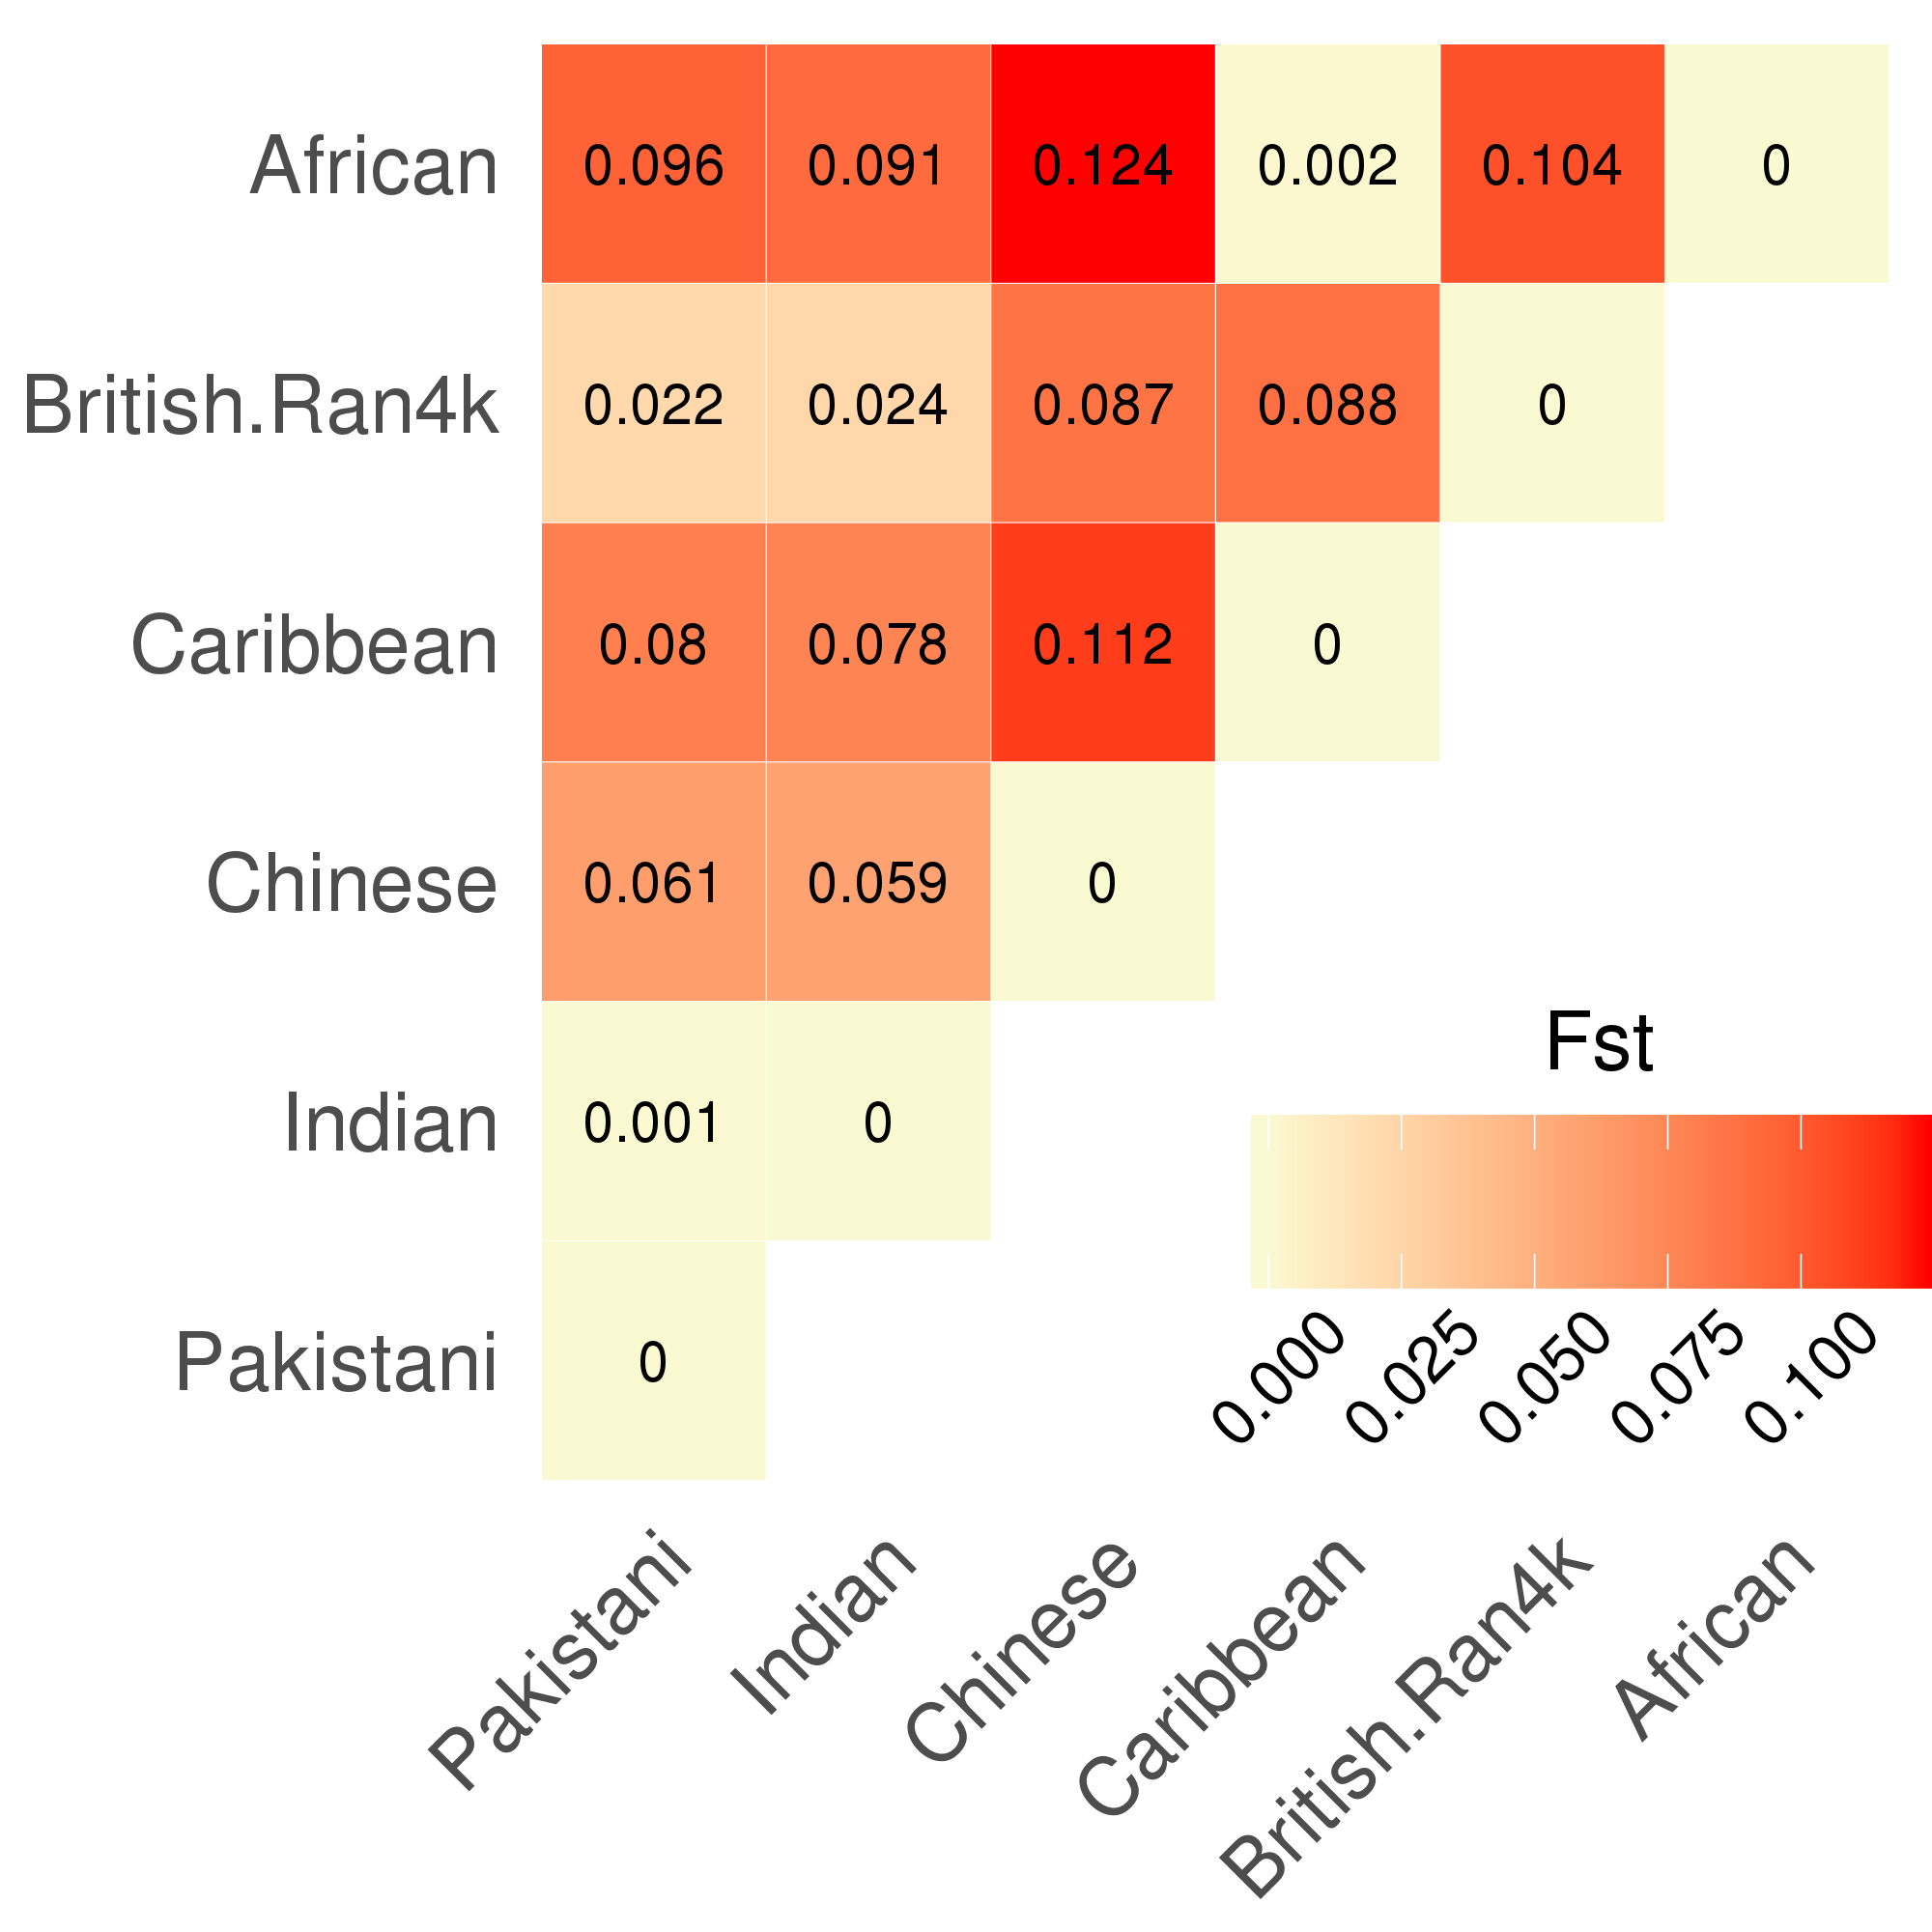
\includegraphics[scale=.5]{Images/Main/InterPath_Main_Figure_Fst_vs2.png}
\caption[TBD]{\textbf{Distribution of pairwise F\textsubscript{ST} across the UKB subsets}. The heatplot shows pairwise F\textsubscript{ST} values between each of our UKB population subsets using our genome-wide SNP data. F\textsubscript{ST} values range from .001 to .124, and we observe typical global patterns (eg African/Caribbean vs. non-African subsets, Chinese vs. non-Asian subsets).}
\label{InterPath-Main-Figure-Fst}
\end{figure}

\begin{figure}[htb]
\centering
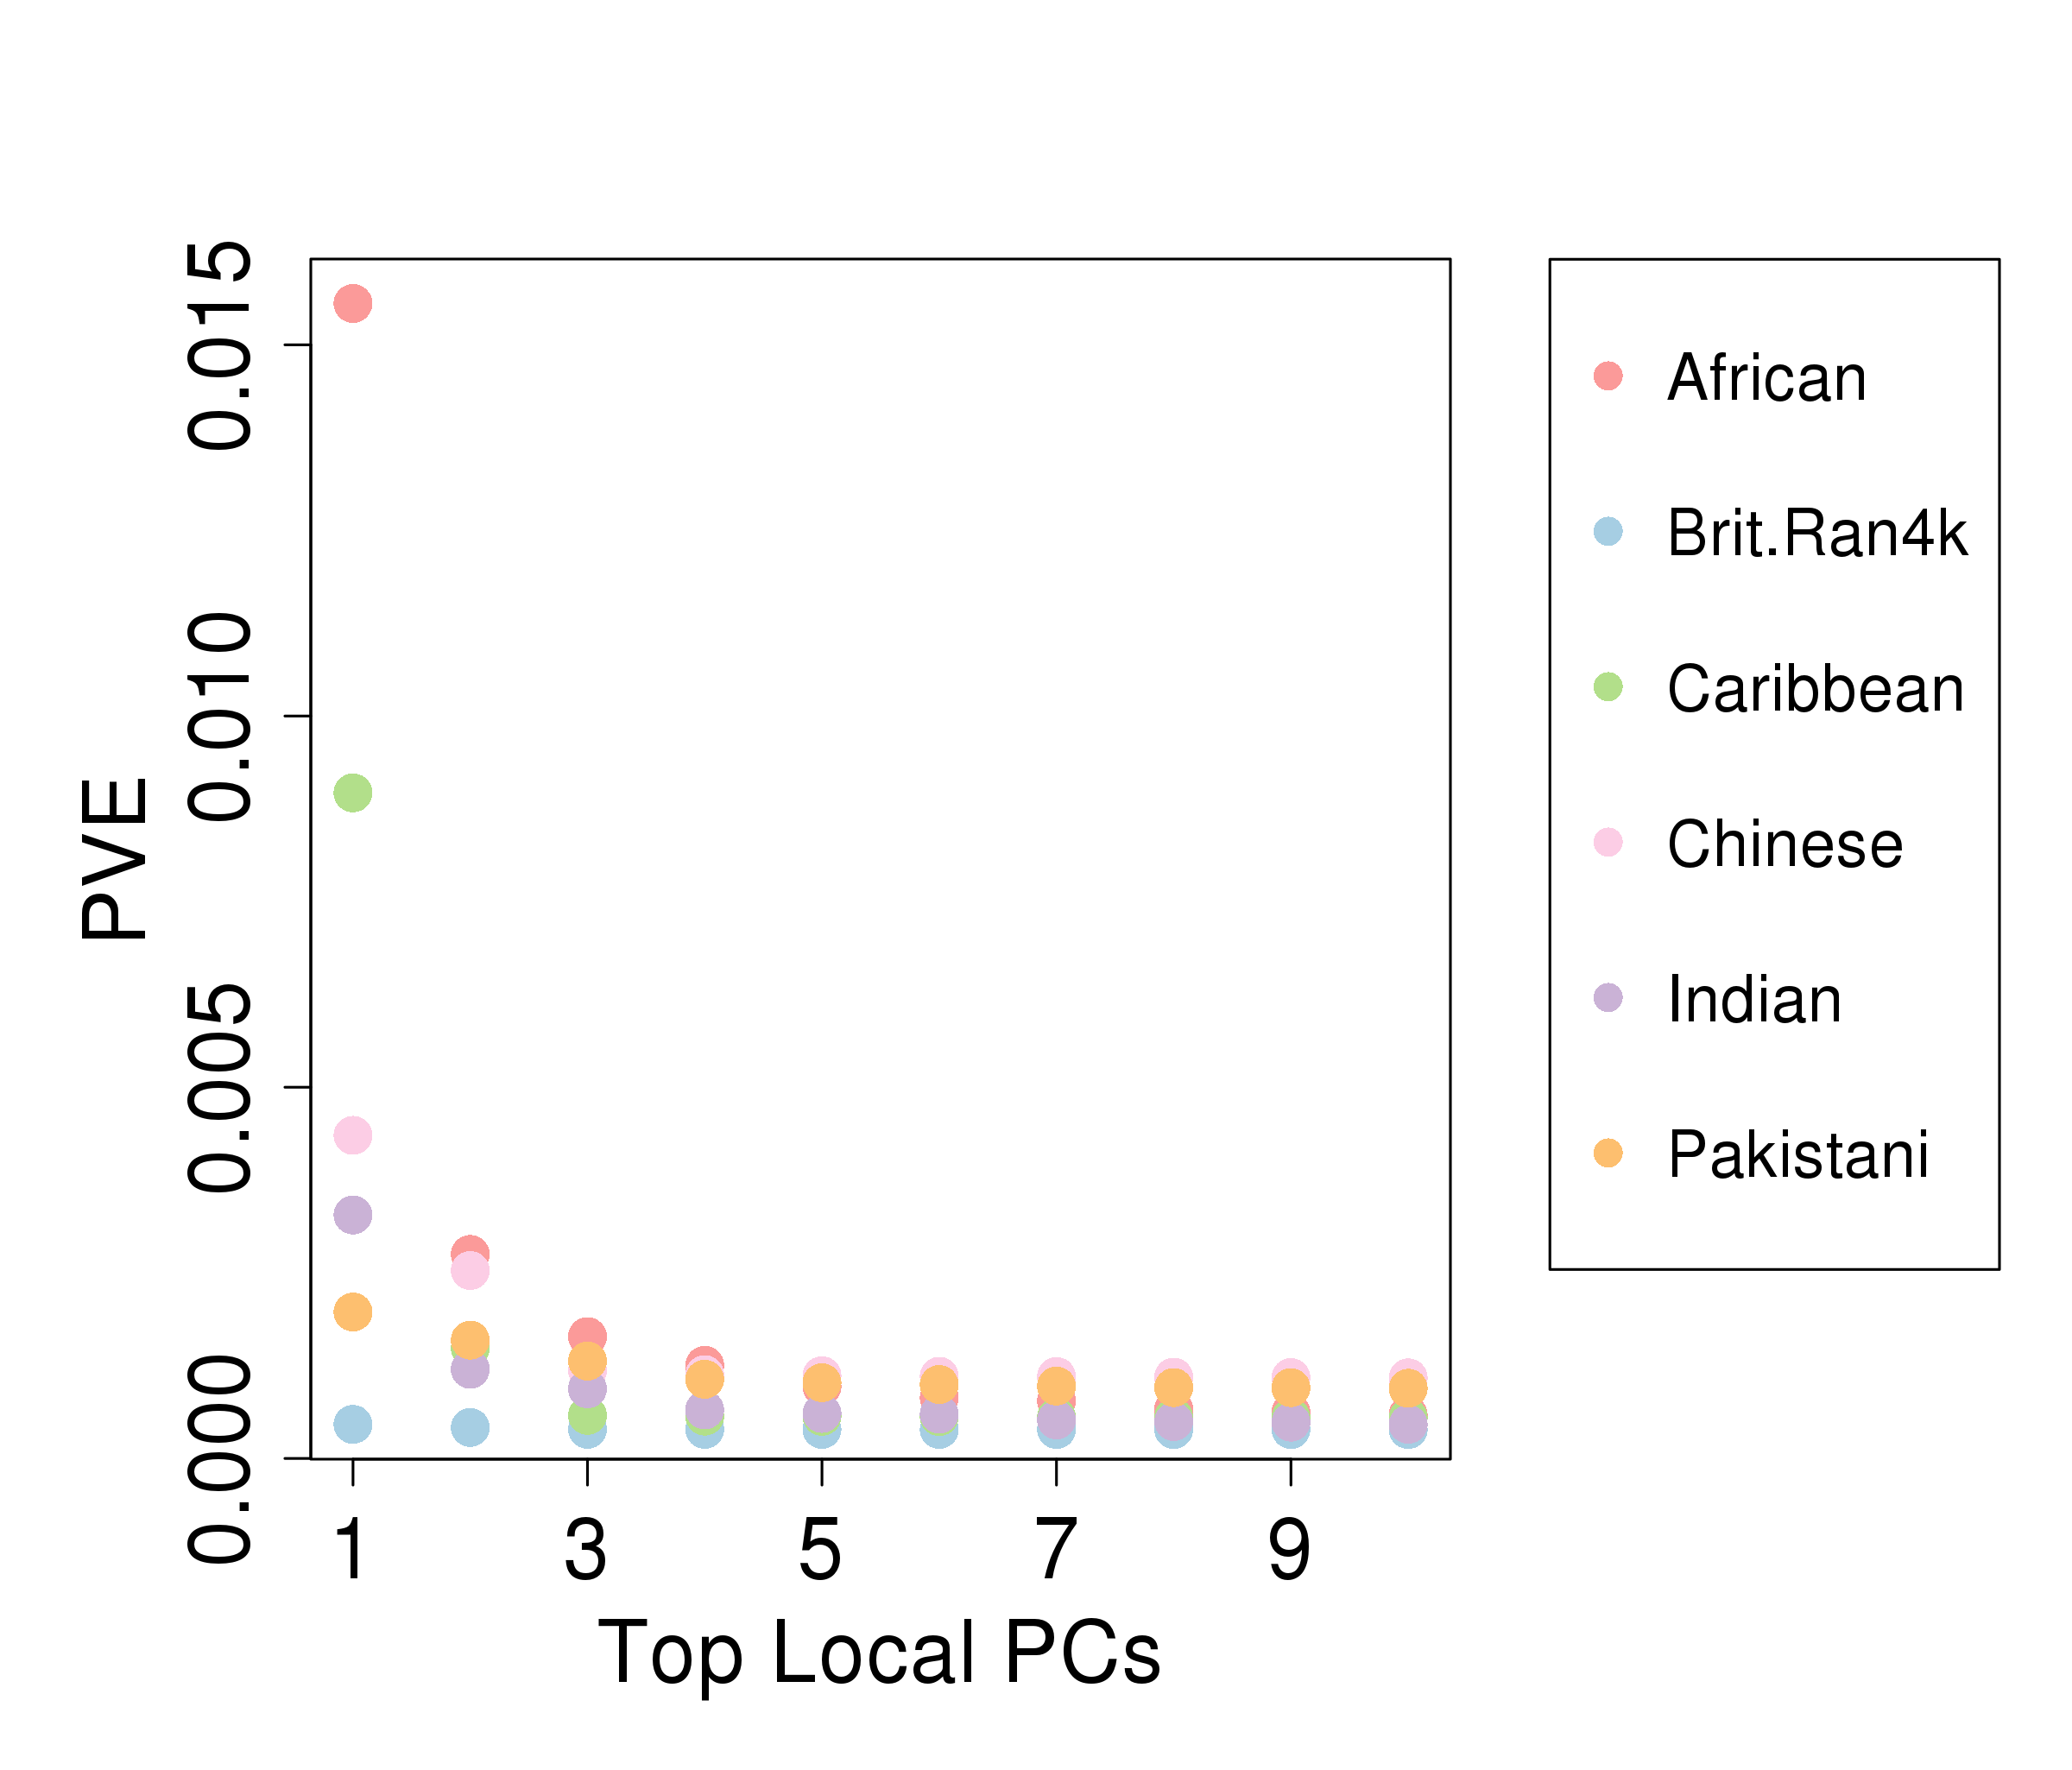
\includegraphics[scale=.5]{Images/Main/InterPath_Main_Figure_Eigenvalues_vs2.png}
\caption[TBD]{\textbf{Distribution of top 10 local principal component PVEs across UKB subsets}. The plot shows the PVE of each of the top 10 local PCs for each of our UKB population subsets. Local here continues to refer to calculating PCs by using each subset separately (versus jointly calculating PCs across all subsets together). We observe that the separation between our subsets in PC1 PVE appears well correlated with the patterns of genome-wide significant MAPIT-R pathways we find for each phenotype and database combination (see Figure \ref{InterPath-Main-Figure-Barplots-KEGG} and  Supplementary Figure \ref{InterPath-Supp-Figure-Barplots-REACTOME}).}
\label{InterPath-Main-Figure-Eigenvalues}
\end{figure}

To take these analyses one step further, we investigated levels of genetic diversity on the pathway-scale as well to see if they are correlated with the MAPIT-R results. To accomplish this, we calculated the mean proportion of pairwise identity-by-state across every pair of individuals on the pathway level. Meaning for a single pathway, we had a metric ranging from 0 to 1 where 1 indicates all pairs of individuals had exactly the same genotypes at every SNP for a given pathway and 0 means all pairs of individuals had completely different genotypes at each of these SNPs. Lower values would then indicate greater levels of genetic diversity for a given pathway within that ancestry subset. Once we had these values, we then compared them against each pathway's MAPIT-R -$\log_{10}$ $p$-value; however, we found there was no relationship between these two metrics (Figure \ref{InterPath-Main-Figure-IBS-African} \& Supplementary Figure \ref{InterPath-Supp-Figure-IBS-AllPops}). This was true across almost every one of our UKB population subsets, phenotype, and pathway database collections. And in general it does not appear that this lack of relationship changes per-ancestry either; directly comparing population subsets against one another shows that the per-pathway IBS proportions follow similar trajectories, shifted only by each population's mean level of IBS (Figure \ref{InterPath-Main-Figure-IBS-AllPopComps-KEGG} \& Supplementary Figure \ref{InterPath-Supp-Figure-IBS-AllPopComps-REACTOME}). Therefore it appears this further supports our previous finding that the signal we are observing in our results is likely not being driven by broadscale levels of genetic variation. Instead, there may be a more cryptic structure and relationship between the genetic variation in each subset and the power to detect epistasis we are observing with MAPIT-R. \textcolor{red}{(I'm assuming we would bring up Lorin's idea of 'higher PC1 values/greater population structure leads to more successful 'population structure correction', hence why we get more signals (removing more noise -> reveals more signal), in the discussion section, not here.}

\begin{figure}[htb]
\centering
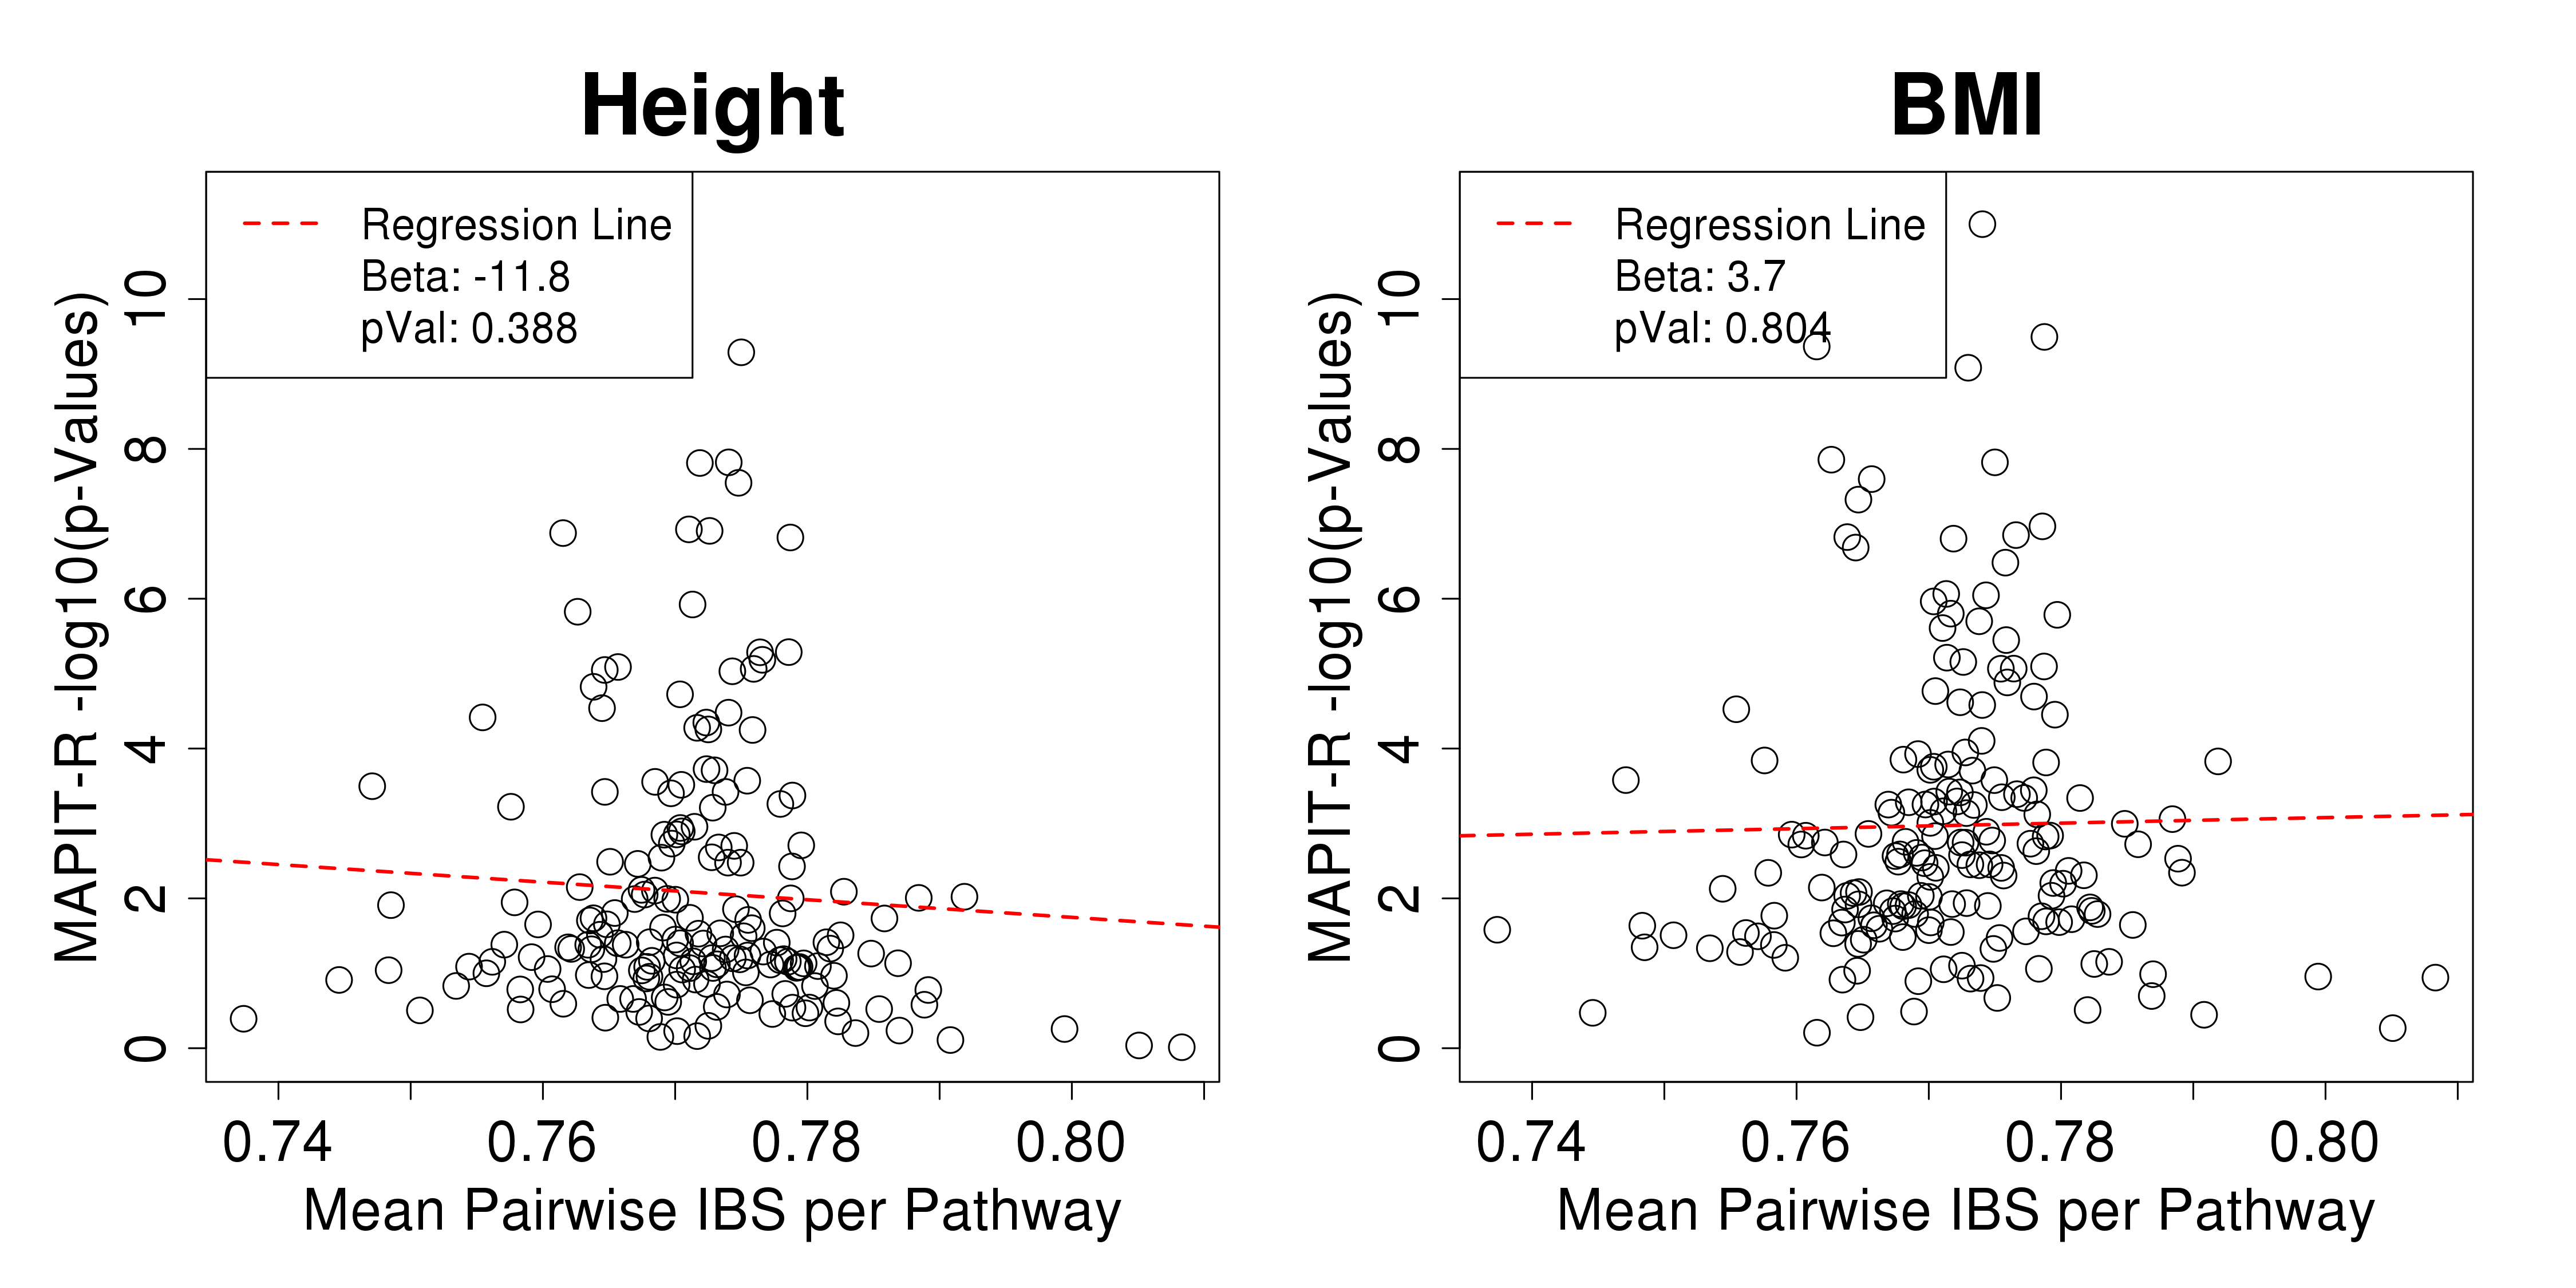
\includegraphics[scale=.35]{Images/Main/InterPath_Main_Figure_IBS_vs3_African.png}
\caption[TBD]{\textbf{Pathway-level genetic diversity versus MAPIT-R results in the African subset and KEGG database}. The figure shows the mean pairwise IBS proportions per pathway plotted against each pathway's MAPIT-R $p$-value for the African subset KEGG height and BMI results. IBS proportions were calculated per pathway by using that pathway's set of SNPs, were calculated pairwise between every set of individuals in the subset, and then averaged across each of these pairs for a final, single summary metric. Results for each phenotype, pathway database, and subset combination can be found in Supplementary Figure \ref{InterPath-Supp-Figure-IBS-AllPops}. We observe across almost every combination no significant relationship between mean pairwise IBS proportion and MAPIT-R $p$-value.}
\label{InterPath-Main-Figure-IBS-African}
\end{figure}

\begin{figure}[htb]
\centering
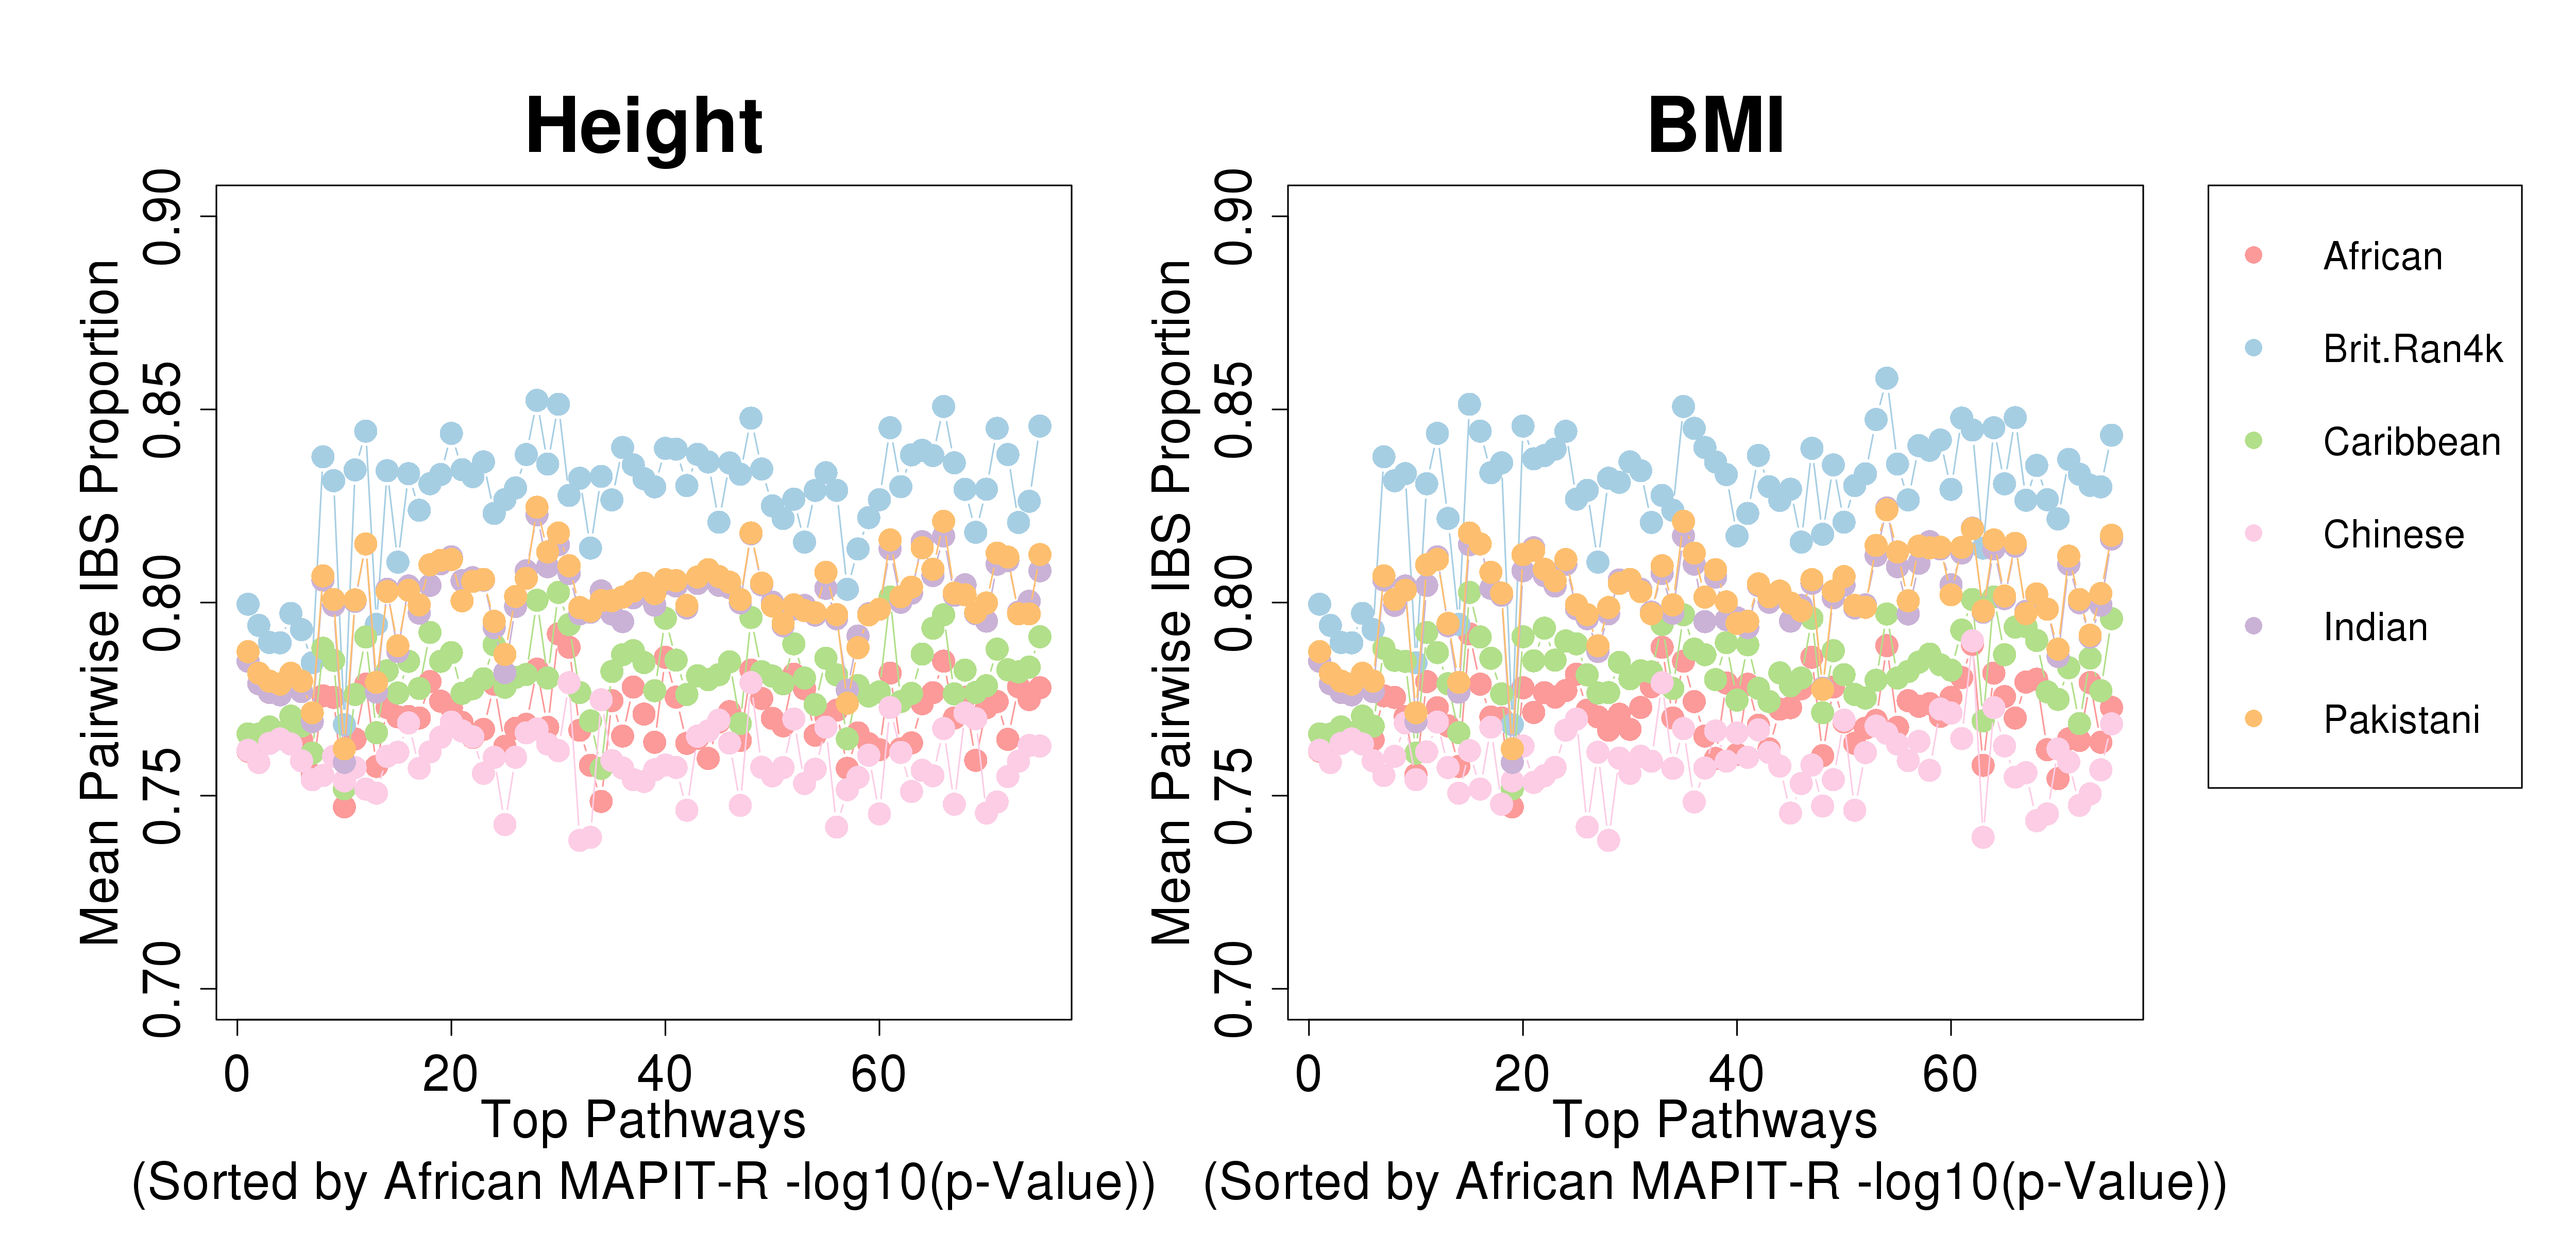
\includegraphics[scale=.35]{Images/Main/InterPath_Main_Figure_IBS_AllPopComps_vs3_KEGG.png}
\caption[TBD]{\textbf{Pathway-level genetic diversity across all UKB subsets for top African MAPIT-R KEGG pathways}. The figure plots the mean pairwise IBS proportions of each UKB subset for the top 75 KEGG pathways (sorted by MAPIT-R African subset $p$-value). Most variation in mean pairwise IBS proportions varies moreso based on the pathways themselves and not on ancestry; subsets differ between one another mostly at the same levels across each pathway. Results for phenotypes in both pathway databases can be see in Supplementary Figure \ref{InterPath-Supp-Figure-IBS-AllPopComps}.}
\label{InterPath-Main-Figure-IBS-AllPopComps-KEGG}
\end{figure}

\section{Discussion}\label{InterPath-Discussion}

\textcolor{blue}{WIP}

Here we present the first exploration of marginal epistasis across multiple human ancestries. Specifically we investigate both single SNP and pathway level marginal epistasis in height and BMI, and present a novel framework for analyzing marginal epistasis in pathways. We find that our African subset is particularly well-powered to detect signals of pathway marginal epistasis, with this subset containing over XX\% of our XX total genome-wide hits. We show that these results are unlikely to be the product of artifactual biases such as SNP count, residual population structure, or genotyping chip. We also show evidence that these results are unlikely to be a product of simply choosing optimal, unrepresentative samples of the full populations. And lastly, we find evidence that cellular signaling and immune-related pathways may be particularly enriched for marginal epistasis, and the proteasome as a protein complex may be enriched for marginal epistatic interactions as well. 

contains an abundance of pathways with statistical significant marginal epistatic interactions,  XX pathways have statistically significant interactions with the rest of the genome, XX (XX\%) of which




\section{Methods}\label{InterPath-Online-Methods}

\subsection{UK BioBank Data}

\subsubsection{Population Subsets}
UK BioBank data was applied for and downloaded from XXX. We first grouped and extracted our multiple population subsets by using self-identified ancestry (`African', `British', `Caribbean', `Chinese', `Indian', `Irish', and `Pakistani'). British random subsets of 4,000 and 10,000 individuals, both the original sets and the additional four rounds of replications, were constructed by randomly choosing initial sets of non-overlapping 4,000 and 10,000 individuals; each round of 4,000 and 10,000 individuals were ensured not to overlap with the previous rounds of the same size of subset. Standard quality control (QC) procedures were employed on each population subset (see Supplementary Note for details). Note that unless stated otherwise, the genetic data used in these analyses were the directly genotyped variant sets from the UKB post-imputation on the University of Michigan Imputation Server \citep{Das2016}; most of the analyses in this manuscript utilized genetic relatedness matrices (GRMs), and GRMs have a stringent requirement of zero genotype missingness. To minimize the loss of SNPs while meeting this threshold we chose to impute missing genotypes while still focusing on just the original set of genotyped variants.

\subsubsection{Phenotypes}

For all the analyses presented in here, height and BMI were our complex traits of interest. Each phenotype was adjusted for age, gender, and assessment center. Following previous pipelines (cite GIANT), each dataset was first divided into male and female subsets. Age was then regressed out within each sex. The resulting residuals were then inverse normalized according to equation \#\# found in the supplement of (citation). These normalized values were then combined back between sexes, and, lastly, assessment center designations \textcolor{red}{(give UKB identifier?)} as detailed by the UKB were regressed out as well. 

\subsubsection{Global Principal Components}

To take into account possible global patterns of population structure, principal components to be used as covariates during analyses were derived by running PCA on our full set of UKB populations. FlashPCA2 was used to run PCA, and as stated, all of our post-QC, post-imputation population files were analyzed together.    

\subsection{PLINK Analyses}

PLINK pairwise epistasis analyses were conducted using PLINK v1.90b4 \citep{Purcell2007}, the `\texttt{-{}-epistasis}' command, and phenotypes that had top 10 global PCs regressed out; PCs were regressed out directly from the phenotypes due to the `\texttt{-{}-epistasis}' function having no explicit form to incorporate covariates. Default values for the `\texttt{-{}-epi1}' and `\texttt{-{}-epi2}' options (0.0001 and 0.01, respectively) were kept. And the PLINK model is as follows:
\begin{equation}
\textbf{y} = \beta_0 + \textbf{x}_1\beta_1 + \textbf{x}_2\beta_2 + \textbf{x}_1*\textbf{x}_2\beta_3    
\end{equation}
where \textbf{y} is once again a $n \times 1$ vector of phenotypes, $\beta_0$ is the y-intercept, $\textbf{x}_1$ is a $n \times 1$ vector of genotypes for SNP 1, $\beta_1$ is the corresponding additive effect size for $\textbf{x}_1$, $\textbf{x}_2$ is a $n \times 1$ vector of genotypes for SNP 2, $\beta_2$ is the corresponding additive effect size for $\textbf{x}_2$, $\textbf{x}_1 * \textbf{x}_2$ is the multiplicative interaction between $\textbf{x}_1$ and $\textbf{x}_2$, and $\beta_3$ is the corresponding effect size for $\textbf{x}_1 * \textbf{x}_2$. Our variable of interest of course is $\beta_3$ and whether this value significantly deviates from 0.  

\subsection{MAPIT Analyses}

MAPIT analyses were conducted using the MAPIT software downloaded from \url{https://github.com/lorinanthony/MAPIT}. MAPIT was run using the phenotypes as previously described and top 10 global PCs as covariates. The 

\noindent `\texttt{MAPIT\_Davies\_Approx}' function was used due to its computational speed up and having large enough sample sizes to properly employ the Davies approximation. 

To test for SNP-level marginal epistasis, we use MAPIT \citep{Crawford2017}. For a full derivation of the MAPIT framework please see \citet{Crawford2017}, but in short MAPIT begins with the following setup:
\begin{equation}
\textbf{y} = \mu + \textbf{x}_k\beta_k + \sum_{l \neq k} \textbf{x}_l\beta_l + \sum_{l \neq k} (\textbf{x}_k \circ \textbf{x}_l)\alpha_l + \boldsymbol{\epsilon}, \quad \boldsymbol{\epsilon} \sim \mathcal{MVN}(\textbf{0}, \tau^{2}\textbf{I})  
\end{equation}

where \textbf{y} is still a $n \times 1$ vector of phenotypes, $\textbf{x}_k$ is a $n \times 1$ vector of genotypes for our SNP of interest $k$, $\beta_k$ is our additive effect size for SNP $k$, $\textbf{x}_l$ is a $n \times 1$ vector of genotypes for every SNP $l$ that is not SNP $k$, $\beta_l$ is our additive effect size for SNP $l$, $(\textbf{x}_k \circ \textbf{x}_l)$ is the Hadamard product between our two SNP genotype vectors, $\alpha_l$ is interaction effect size, $\boldsymbol{\epsilon}$ is a $n \times 1$ vector of random effects which follow a multivariate normal distribution with mean $\textbf{0}$ and covariance matrix equal to variance effect $\tau$ times the $n \times n$ identity matrix $\textbf{I}$. In this model our parameter of interest would be $\alpha_l$, whether there is any significant interaction between our SNP of interest $k$ and of the remaining SNPs in the genome. However, as one might expect, the number of parameters in this model far exceeds the number of samples (ie $p >> n$), therefore making the solution indeterminable. To overcome this, MAPIT moves this setup into a linear mixed model framework and make the problem a variance component one. To do this, we put normal random priors on each of our effect sizes ($\beta_k$, $\beta_l$, and $\alpha_l$), and redefine our model as follows:
\begin{align}
    & \textbf{y} = \mu + \textbf{x}_k\beta_k + \textbf{m}_k + \textbf{g}_k + \boldsymbol{\epsilon} \\
    \textbf{m}_k \sim \mathcal{MVN}(\textbf{0}, &\omega^{2}\textbf{K}_k) \quad \textbf{g}_k \sim \mathcal{MVN}(\textbf{0}, \sigma^{2}\textbf{G}_k) \quad \boldsymbol{\epsilon} \sim \mathcal{MVN}(\textbf{0}, \tau^{2}\textbf{I}) \nonumber 
\end{align}
where $\textbf{m}_k$ and $\textbf{g}_k$ are both random effects that follow multivariate normal distributions, $\omega$ and $\sigma$ are their respective variance components, $\textbf{K}_k = \textbf{X}_{-k}\textbf{X}^{\textbf{T}}_{-k}/(p-1)$, the genetic relatedness matrix (GRM) constructed from all SNPs available aside from SNP $k$, and $\textbf{G} = \textbf{D}_k\textbf{K}_k\textbf{D}_k$, a GRM based on pairwise interaction terms between the $k$\textsuperscript{th} variant and all other variants. Here, we denote $\textbf{D}_k =$ diag$(\textbf{x}_k)$ to be an $n \times n$ diagonal matrix with the genotype vector $\textbf{x}_k$ as its diagonal elements. Our parameter of interest here is $\sigma$ and whether it is significantly larger from 0; a significant deviation would represent there exist some subset of genetic interactions between $k$ and the rest of the genome.

\subsection{MAPIT-R Model}

We describe the framework for ``\underline{Inter}actions in \underline{Path}way'' (MAPIT-R) analysis in detail here. The key goal of this method is to identify crosstalk between signaling pathways in GWAS, without having to explicitly model all possible higher-order interactions. In general, consider a pathway which is defined by a set of SNPs found within the regulatory regions of genes in that pathway. We will denote these variants with the set of indices $\mathcal{R} = (r_1,\ldots,r_p)$. Begin by considering the following partitioned linear regression model,
\begin{equation}\label{LM}
\by = \mu\bm{1}+\sum_{r\in \mathcal{R}}\bx_r\beta_{r}+\sum_{s\not\in \mathcal{R}}\bx_s\beta_{s}+\bvarepsilon, \quad \bvarepsilon\sim \mathcal{N}(\mathbf{0}, \tau^2\bI),
\end{equation}
where $\by$ is an $n$-dimensional vector of quantitative phenotypes for $n$ individuals; $\mu$ is an intercept term with an $n$-dimensional vector of ones; $\bx_r$ and $\bx_s$ are $n$-dimensional genotype vectors for variants that lie within and outside the regulatory region $\mathcal{R}$, respectively; $\beta_r$ and $\beta_s$ are the corresponding additive effect sizes; $\bvarepsilon$ is an $n$-vector of residual errors; $\tau^2$ is the residual error variance; $\bI$ denotes the identity matrix; and $\mathcal{N}(\bullet,\bullet)$ denotes a multivariate normal distribution. Here, we also assume that the genotypic vectors have been centered and standardized to have mean 0 and standard deviation 1.

Because we consider scenarios where there are more variants than samples, we need to specify additional modeling assumptions in Equation \eq{LM} to make the rest of the model identifiable. In particular, we recall previous approaches and assume that the individual effect sizes follow univariate normal distributions, or $\beta_r \sim \mathcal{N}(0, \omega^2/p)$ and $\beta_s \sim \mathcal{N}(0, \sigma^2/(l-p))$, where $l$ is the number of total number of all SNPs \citep{Crawford2017}. With the assumption of normally distributed effect sizes, the model defined in Equation \eq{LM} is equivalent to a variance component model where $\bg\sim \mathcal{N}(\bm{0}, \omega^2\bK)$ with $\bK=\bX_{\mathcal{R}}\bX_{\mathcal{R}}^{\T}/p$ being the genetic relatedness matrix computed using genotypes from all variants within the signaling pathway of interest; and $\wt\bg\sim \mathcal{N}(\bm{0}, \nu^2\wt\bK)$ with $\wt\bK=\bX_{-\mathcal{R}}\bX_{-\mathcal{R}}^{\T}/(l-p)$ representing a relatedness matrix computed using all other variants. Note that $\bg$ may be interpreted as a pathway's additive effect, while $\wt\bg$ denotes its polygenic background. 

To complete the specification of the MAPIT-R methodology, we lastly assume an additional random effect $\bu$ which models the summation of all pairwise interaction effects between a given signaling pathway variant and all other pathways. In this work, we limit ourselves to the case of finding second order crosstalk relationships between pathways --- although, extensions to higher-order interactions is straightforward \citep{Crawford2017}. Altogether, this results in the following linear mixed model
\begin{equation}
\by = \mu\bm{1}+ \bg +\wt\bg+\bu+\bvarepsilon,\\ 
\bg\sim \mathcal{N}(\bm{0}, \omega^2\bK), \quad \wt\bg\sim \mathcal{N}(\bm{0},
\nu^2\wt\bK),\\ 
\bu\sim\mathcal{N}(\bm{0},\sigma^2\bQ), \quad \bvarepsilon\sim \mathcal{N}(\mathbf{0}, \tau^2\bI).\label{LMM}
\end{equation}
Here, the $\bQ = \bK\circ\wt\bK$ is represents a second-order interaction relationship matrix, and is obtained by using the Hadamard product (i.e.~the squaring of each element) between the pathway specific relatedness matrix and its corresponding polygenic background. Note that the formulation of MAPIT-R in Equation \eq{LMM} can easily be extended to accommodate other fixed effects (e.g.~age, sex, or genotype principal components), as well as other random effects terms that can be used to account for sample non-independence due to other genetic or common environmental factors.

%Note that we make the assumption that each $\bg_k^{(l)}\sim \mbox{MVN}(\bm{0}, \sigma_{l}^2\bK^l_k)$, where the baseline covariance matrix $\bK_k=\bX_{-\mathcal{R}}\bX_{-\mathcal{R}}^{\T}/p_k$ is the conventional genetic relatedness matrix computed using genotypes from all $p_k$ variants outside of the region $\mathcal{R}$. Here, we use the power factor $l$ to denote the order of interaction (epistatic) effects that are accounted for within the model. For example, when $l=2$, $\mathbf{K}_k^2 = \mathbf{K}_k\circ\mathbf{K}_k$ represents a pairwise interaction relationship matrix, and is obtained by using the Hadamard product (i.e.~the squaring of each element) of the linear kernel matrix with itself \citep{Henderson:1985aa,Ronnegard:2008aa,Jiang:2015aa}. In this case, $\mathbf{K}_k^2$ denotes the marginal second order epistatic effect of the $k$\textsuperscript{th} functional marker under the polygenic background of all other markers. It is important to note that each $\bK_k^{l}$ changes with every new gene, protein, or pathway $k$ that is considered.

\subsection{Hypothesis Testing for Interaction Effects}

Our goal is to identify signaling pathways that have significant non-zero interaction effects on a given phenotype. To do so, we examine each $r$-th pathway of interest in turn, and test the null hypothesis in Equation \eqref{LMM} that $\text{H}_0: \sigma^2=0$. The variance component $\sigma^2$ effectively captures the total interaction effects between the $r$-th pathway and all other pathways. We refer to this as the marginal interaction effect for the $r$-th pathway. To do so, we make use of the MQS method for parameter estimation and hypothesis testing \citep{Zhou2017}. Briefly, MQS is based on the computationally efficient method of moments and produces estimates that are mathematically identical to the Haseman-Elston (HE) cross-product regression \citep{Haseman1972}. To estimate the variance components with MQS, we first multiply Equation \eq{LMM} by a projection (hat) matrix onto the null space of the intercept term $\mu$, where $\bH=\bI-\bm{1}(\bm{1}^{\T}\bm{1})^{-1}\bm{1}^{\T}$. After this projection procedure, we obtain a simplified linear mixed model 
\begin{equation}
\by^*_r = \bg^*_r +\wt\bg^*_r+\bu^*_r+\bvarepsilon^*_r\\ 
\bg_r\sim \mathcal{N}(\bm{0}, \omega^2\bK^*_r), \quad \wt\bg_r\sim \mathcal{N}(\bm{0}, \nu^2\wt\bK^*_r),\\ \bu_r\sim\mathcal{N}(\bm{0},\sigma^2\bQ^*_r), \quad \bvarepsilon_r\sim \mathcal{N}(\mathbf{0}, \tau^2\bH) \label{LMM2}
\end{equation}
where $\by^*_r=\bH\by$; $\bg^*_r = \bH\bg_r$; $\bK^*_r = \bH\bK_r\bH$; $\wt\bg_r^* = \bH\wt\bg_r$; $\wt\bK_r^* = \bH\wt\bK_r\bH$; $\bu^*_r = \bH\bu_r$; $\bQ^*_r = \bH\bQ_r\bH$; and $\bvarepsilon_r^* = \bH_r\bvarepsilon$, respectively. Then for each pathway considered, the MQS estimate for the marginal interaction effect is computed as
\begin{equation}
\wh\sigma^2 = \by^{*\T}_r\bA_r\by
\end{equation}
where $\bA_{r} = (\bS_r^{-1})_{31}\bK_r^*+(\bS_r^{-1})_{32}\wt\bK_r^*+(\bS_r^{-1})_{33}\bQ^*_r+(\bS_r^{-1})_{34}\bH$ with elements $(\bS_r)_{jk} = \tr(\bSigma_{rj} \bSigma_{rk})$ for the covariances matrices subscripted as $[\bSigma_{r1}; \bSigma_{r2}; \bSigma_{r3}; \bSigma_{r4}]  = [\bK^*_r; \wt\bK^*_r; \bQ^*_r; \bH]$. Here, $\tr(\bullet)$ is used to denote the matrix trace function. It has been shown that, under MQS, a given marginal variance component estimate $\wh\sigma^2$ follows a mixture of chi-square distributions under the null hypothesis \citep{Crawford2017}. Namely, $\wh\sigma^2 \sim \sum_{i=1}^{n}\lambda_{i}\chi^2_{1,i}$, where $\chi^2_{1}$ are chi-square random variables with one degree of freedom and $(\lambda_{1},\ldots,\lambda_{n})$ are the eigenvalues of the matrix 
\begin{equation*}
\left(\wh\omega^2_{0}\bK^*_r+\wh\nu^2_{0}\wt\bK^*_r+\wh\tau^2_{0}\bH\right)^{1/2} \bA_{r}\left(\wh\omega^2_{0}\bK^*_r+\wh\nu^2_{0}\wt\bK^*_r+\wh\tau^2_{0}\bH\right)^{1/2}
\end{equation*}
with $(\wh\omega^2_{0},\wh\nu^2_{0},\wh\tau^2_{0})$ being the MQS estimates of $(\omega^2,\nu^2,\tau^2)$ under the null hypothesis. Several approximation and exact methods have been suggested to obtain p-values under the distribution of $\wh\sigma^2$. One frequented choice is Davies exact method \citep{Davies1980,Wu2011}. 

%\subsection*{Hypothesis Testing for Overall Associations}

%FORCE also provides an option for summarizing overall marker enrichment. Here, we assume that we have already computed the $q$ marginal effect p-values for genetic marker $k$, denoted as $\wh\bp_k = (\wh p_{k1},\ldots,\wh p_{kq})$. Let $\wh\balpha_k^* = F^{-1}(\wh\bp_k)$ be the transformed test statistic where $F^{-1}$ is the inverse of the cumulative distribution function (CDF) of the standard chi-square $\chi^2_1$. We follow previous works and define the sum of the correlated chi-square variables for a given functional genomic marker as \citep{Nakka:2016aa}
%\begin{equation}
%\bar{\alpha}_k^* = \sum_{l=1}^{q}\wh\alpha_{k,l}^*.\label{Comp}
%\end{equation}
%(NOTE: Follow the rest of the language from methods in PEGASUS here).

\section{URLs}\label{InterPath-URLs}

MAPIT: \url{https://github.com/lorinanthony/MAPIT}
MAPIT-R: \url{https://github.com/mturchin20/MAPIT-R}

\section{Acknowledgments}\label{InterPath-Acknowledgments}

This material is based upon work supported by the National Science Foundation under Grant No. DMS-1439786 while G.D. was in residence at the Institute for Computational and Experimental Research in Mathematics in Providence, RI, during the model and dimension reduction in uncertain and dynamic systems program.

\section{Author Contributions}\label{InterPath-Author-Contributions}

\section{Competing Interests}\label{InterPath-Competing-Interests}

\nolinenumbers

\begingroup
\bibliographystyle{apalike}
\setstretch{1.0}
\bibliography{Main}
\endgroup









\iffalse

SCRAP

Information idea about creating random 'pathways' that have either the same number of genes or SNPs to show that it has to be the *right* collection of information/materials to get the same amount of significance

\subsubsection{Power Gained from Proper Pathway Definitions}

Running a GWAS of height and BMI on each of our population subsets with PLINK, we find only one genome-wide significant hit (Figure \ref{InterPath-Main-Figure-GWAS-Height} \& Supplementary Figure \ref{InterPath-Supp-Figure-GWAS-BMI}). And further similarly to before, we also find a handful of marginally significant variants. More interestingly however, we now ask how similar the MAPIT and GWAS results are. And indeed, comparing the two sets of genome-wide analyzes, we see a wide range of different genetic architecture patterns being represented (Figure \ref{InterPath-Main-Figure-MAPITvsGWAS-AfrHght} \& Supplementary Figure \ref{InterPath-Supp-Figure-MAPITvsGWAS}). Focusing on the African subset and height, we find 49 SNPs that are only marginally significant in MAPIT, 50 SNPs that are only marginally significant in the GWAS, and 0 SNPs that are marginally significant in both tests. Despite the lack of power to identify genome-wide significant results, we still see a strong representation of the partition of additive and epistatic effects in our results. 

\begin{figure}[htbp]
\centering
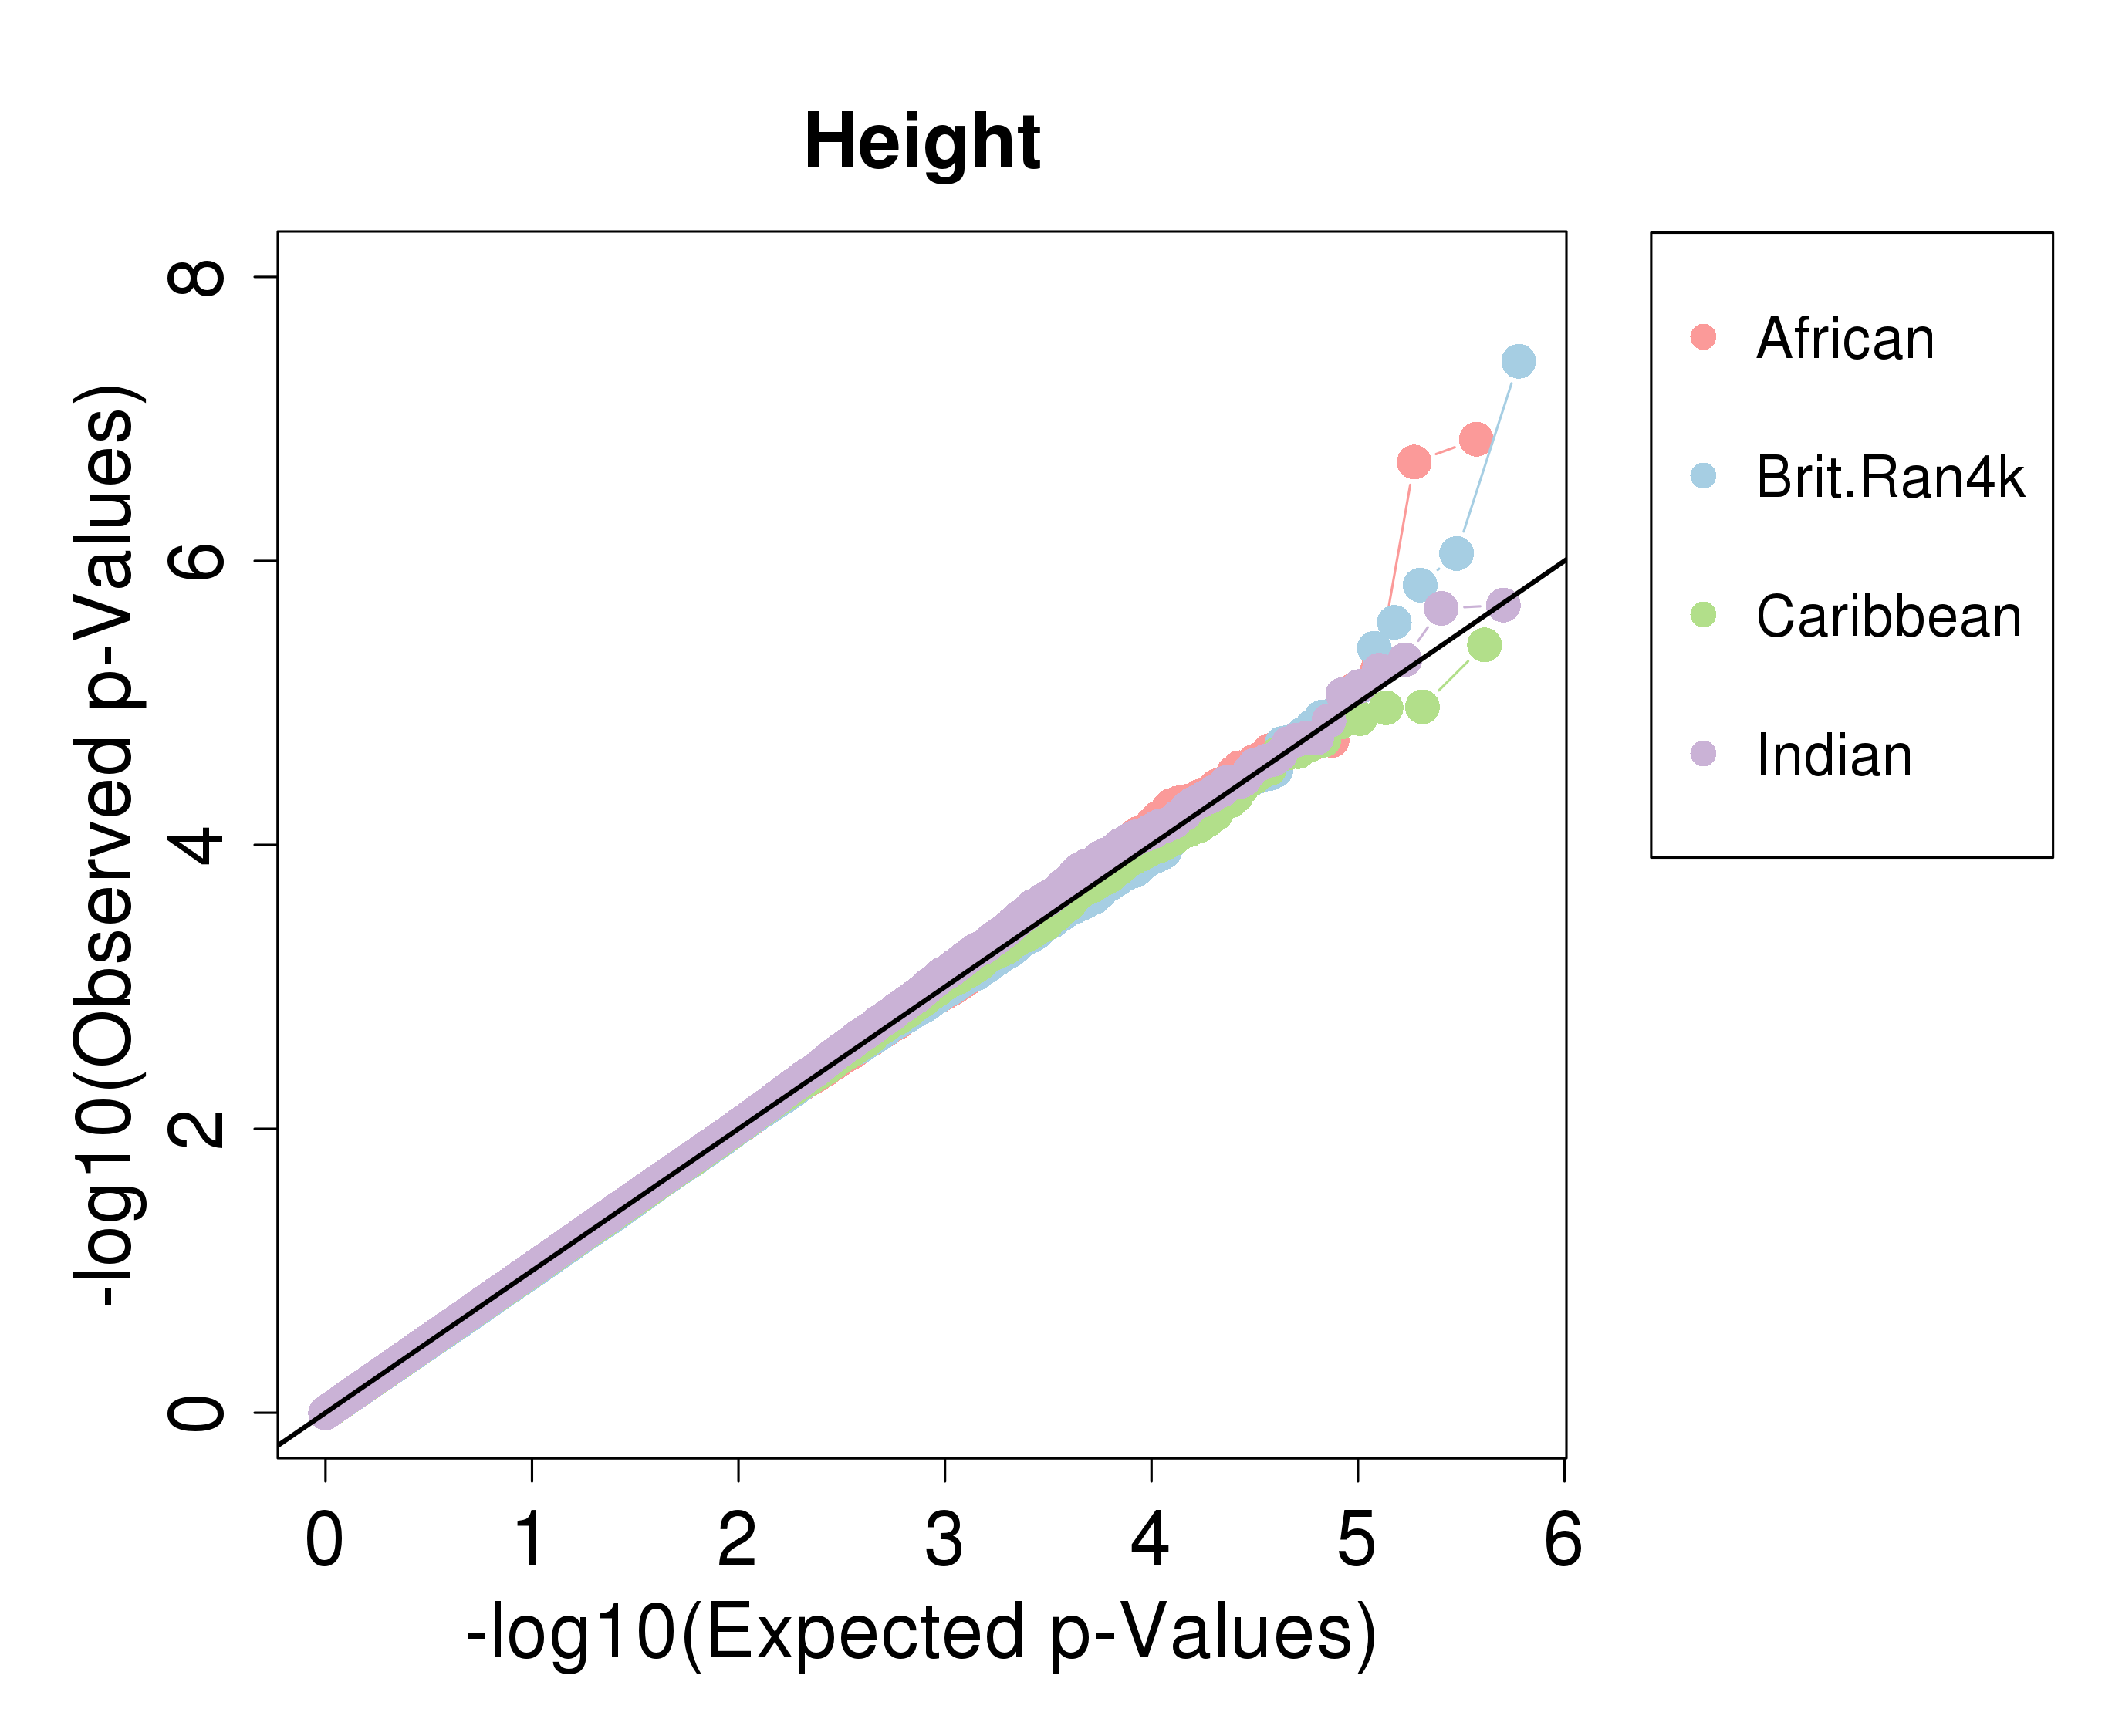
\includegraphics[scale=.35]{Images/Main/InterPath_Main_Figure_GWAS_vs2_Height.png}
\caption[TBD]{\textbf{GWAS Results QQ-Plots}.}
\label{InterPath-Main-Figure-GWAS-Height}
\end{figure}

\begin{figure}[htbp]
\centering
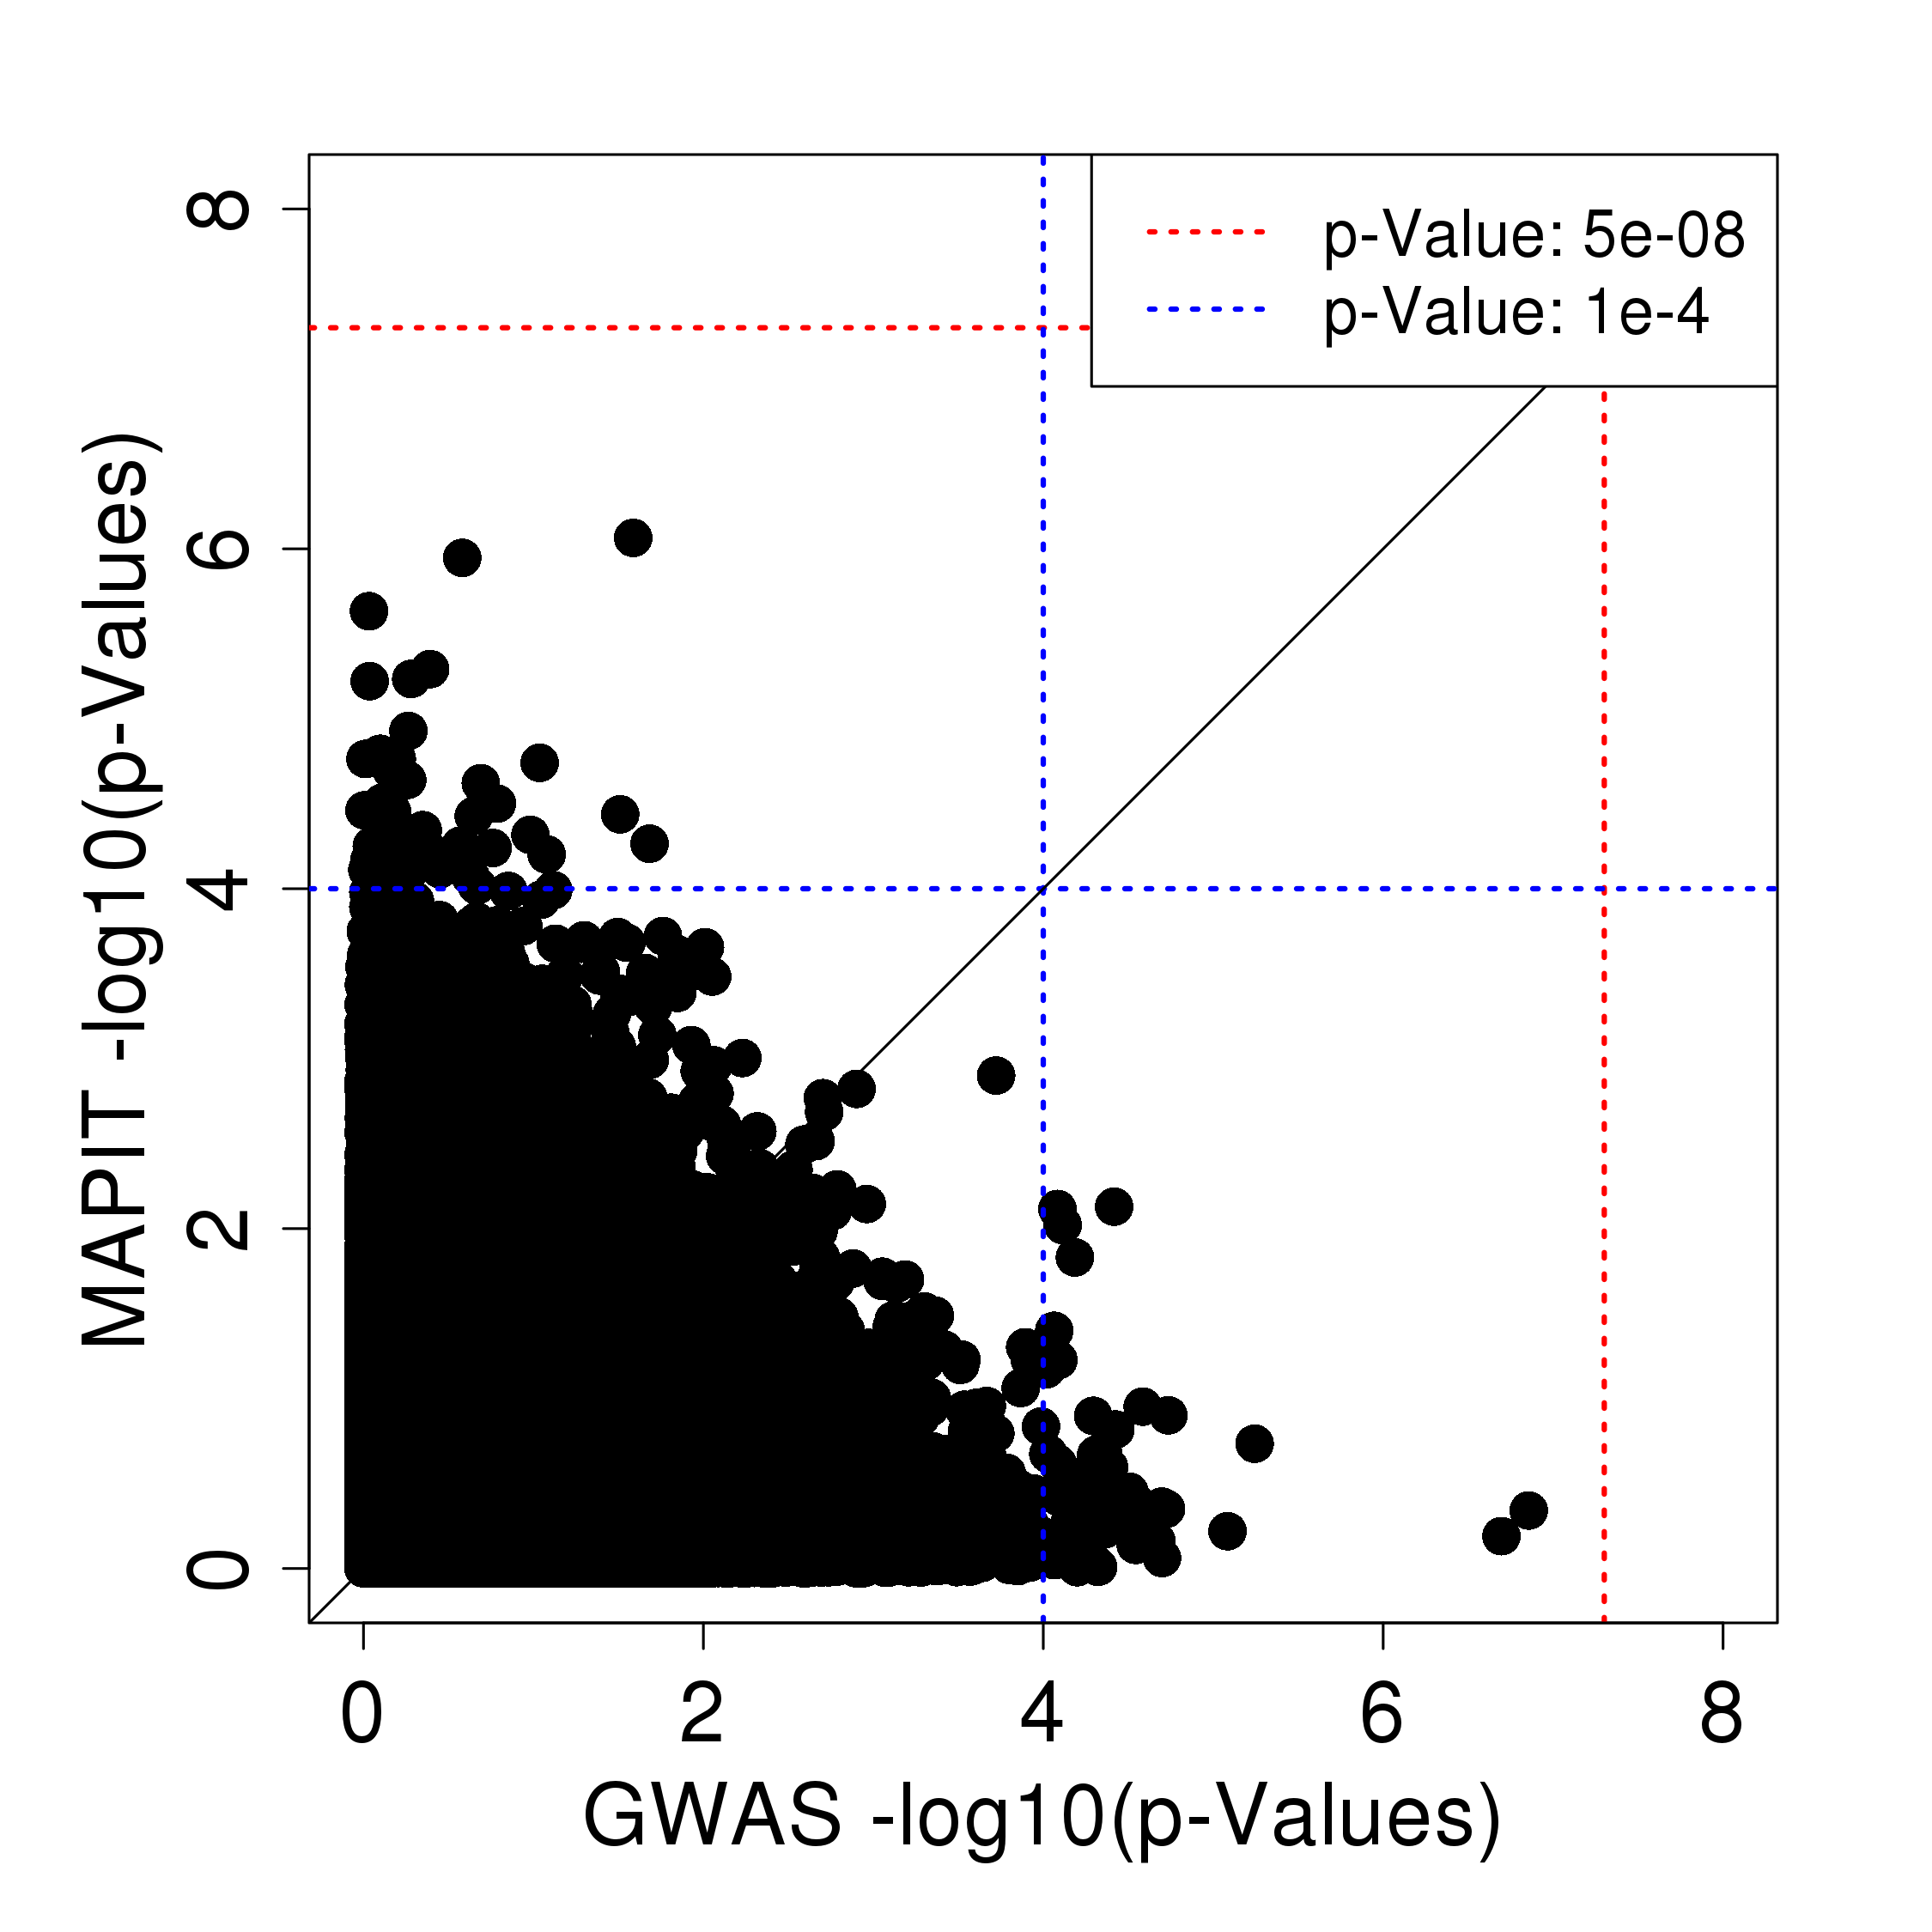
\includegraphics[scale=.35]{Images/Main/InterPath_Main_Figure_MAPITvsGWAS_vs2_AfrHght.png}
\caption[TBD]{\textbf{MAPIT vs. GWAS Results}.}
\label{InterPath-Main-Figure-MAPITvsGWAS-AfrHght}
\end{figure}

\textcolor{red}{(NOTE: below is what we were expecting for these results. But as you can see, the GIANT height/bmi results don't align in the way were anticipating. They are more spread out between height and BMI. I have checked though that the GIANT p-values of these top 500 SNPs are more correlated with our GWAS p-values than our MAPIT p-values (like ~.17 vs. .05). 
I think one alternative approach to this section is to angle instead as: 'we do not have power to even see a difference in GWAS vs. MAPIT as we were anticipating, thus indicating our real need to increase power. Hence, we moved forward with a method that we believed was going to accomplish that').}

To help further get a sense of whether these results are revealing patterns in true biology, we also annotated the top 500 SNPs with the most significant height and BMI GWAS $p$-values from the 2018 GIANT and UKB meta-analysis \cite{Yengo2018} in both our GWAS and MAPIT results. As expected, these 500 SNPs are heavily represented among the tail end of the most significant GWAS results, but maybe less expected is just how insignificant these SNPs appear on the MAPIT list of top results (\textcolor{red}{Supplementary Table -- listing differences in ranking of these 500 SNPs between GWAS and MAPIT}). In fact looking across the genome it is easy to see how different the relative ranking of SNPs are between the GWAS and MAPIT results (Figures \ref{InterPath-Main-Figure-MAPITvsGWAS-Manhattan}D \& \ref{InterPath-Main-Figure-MAPITvsGWAS-Manhattan}E). It is clear that even with our limited sample sizes, differences in the trends of importance of additive versus epistatic signals can be observed among marginally significant SNPs.  

\begin{figure}[htbp]
\centering
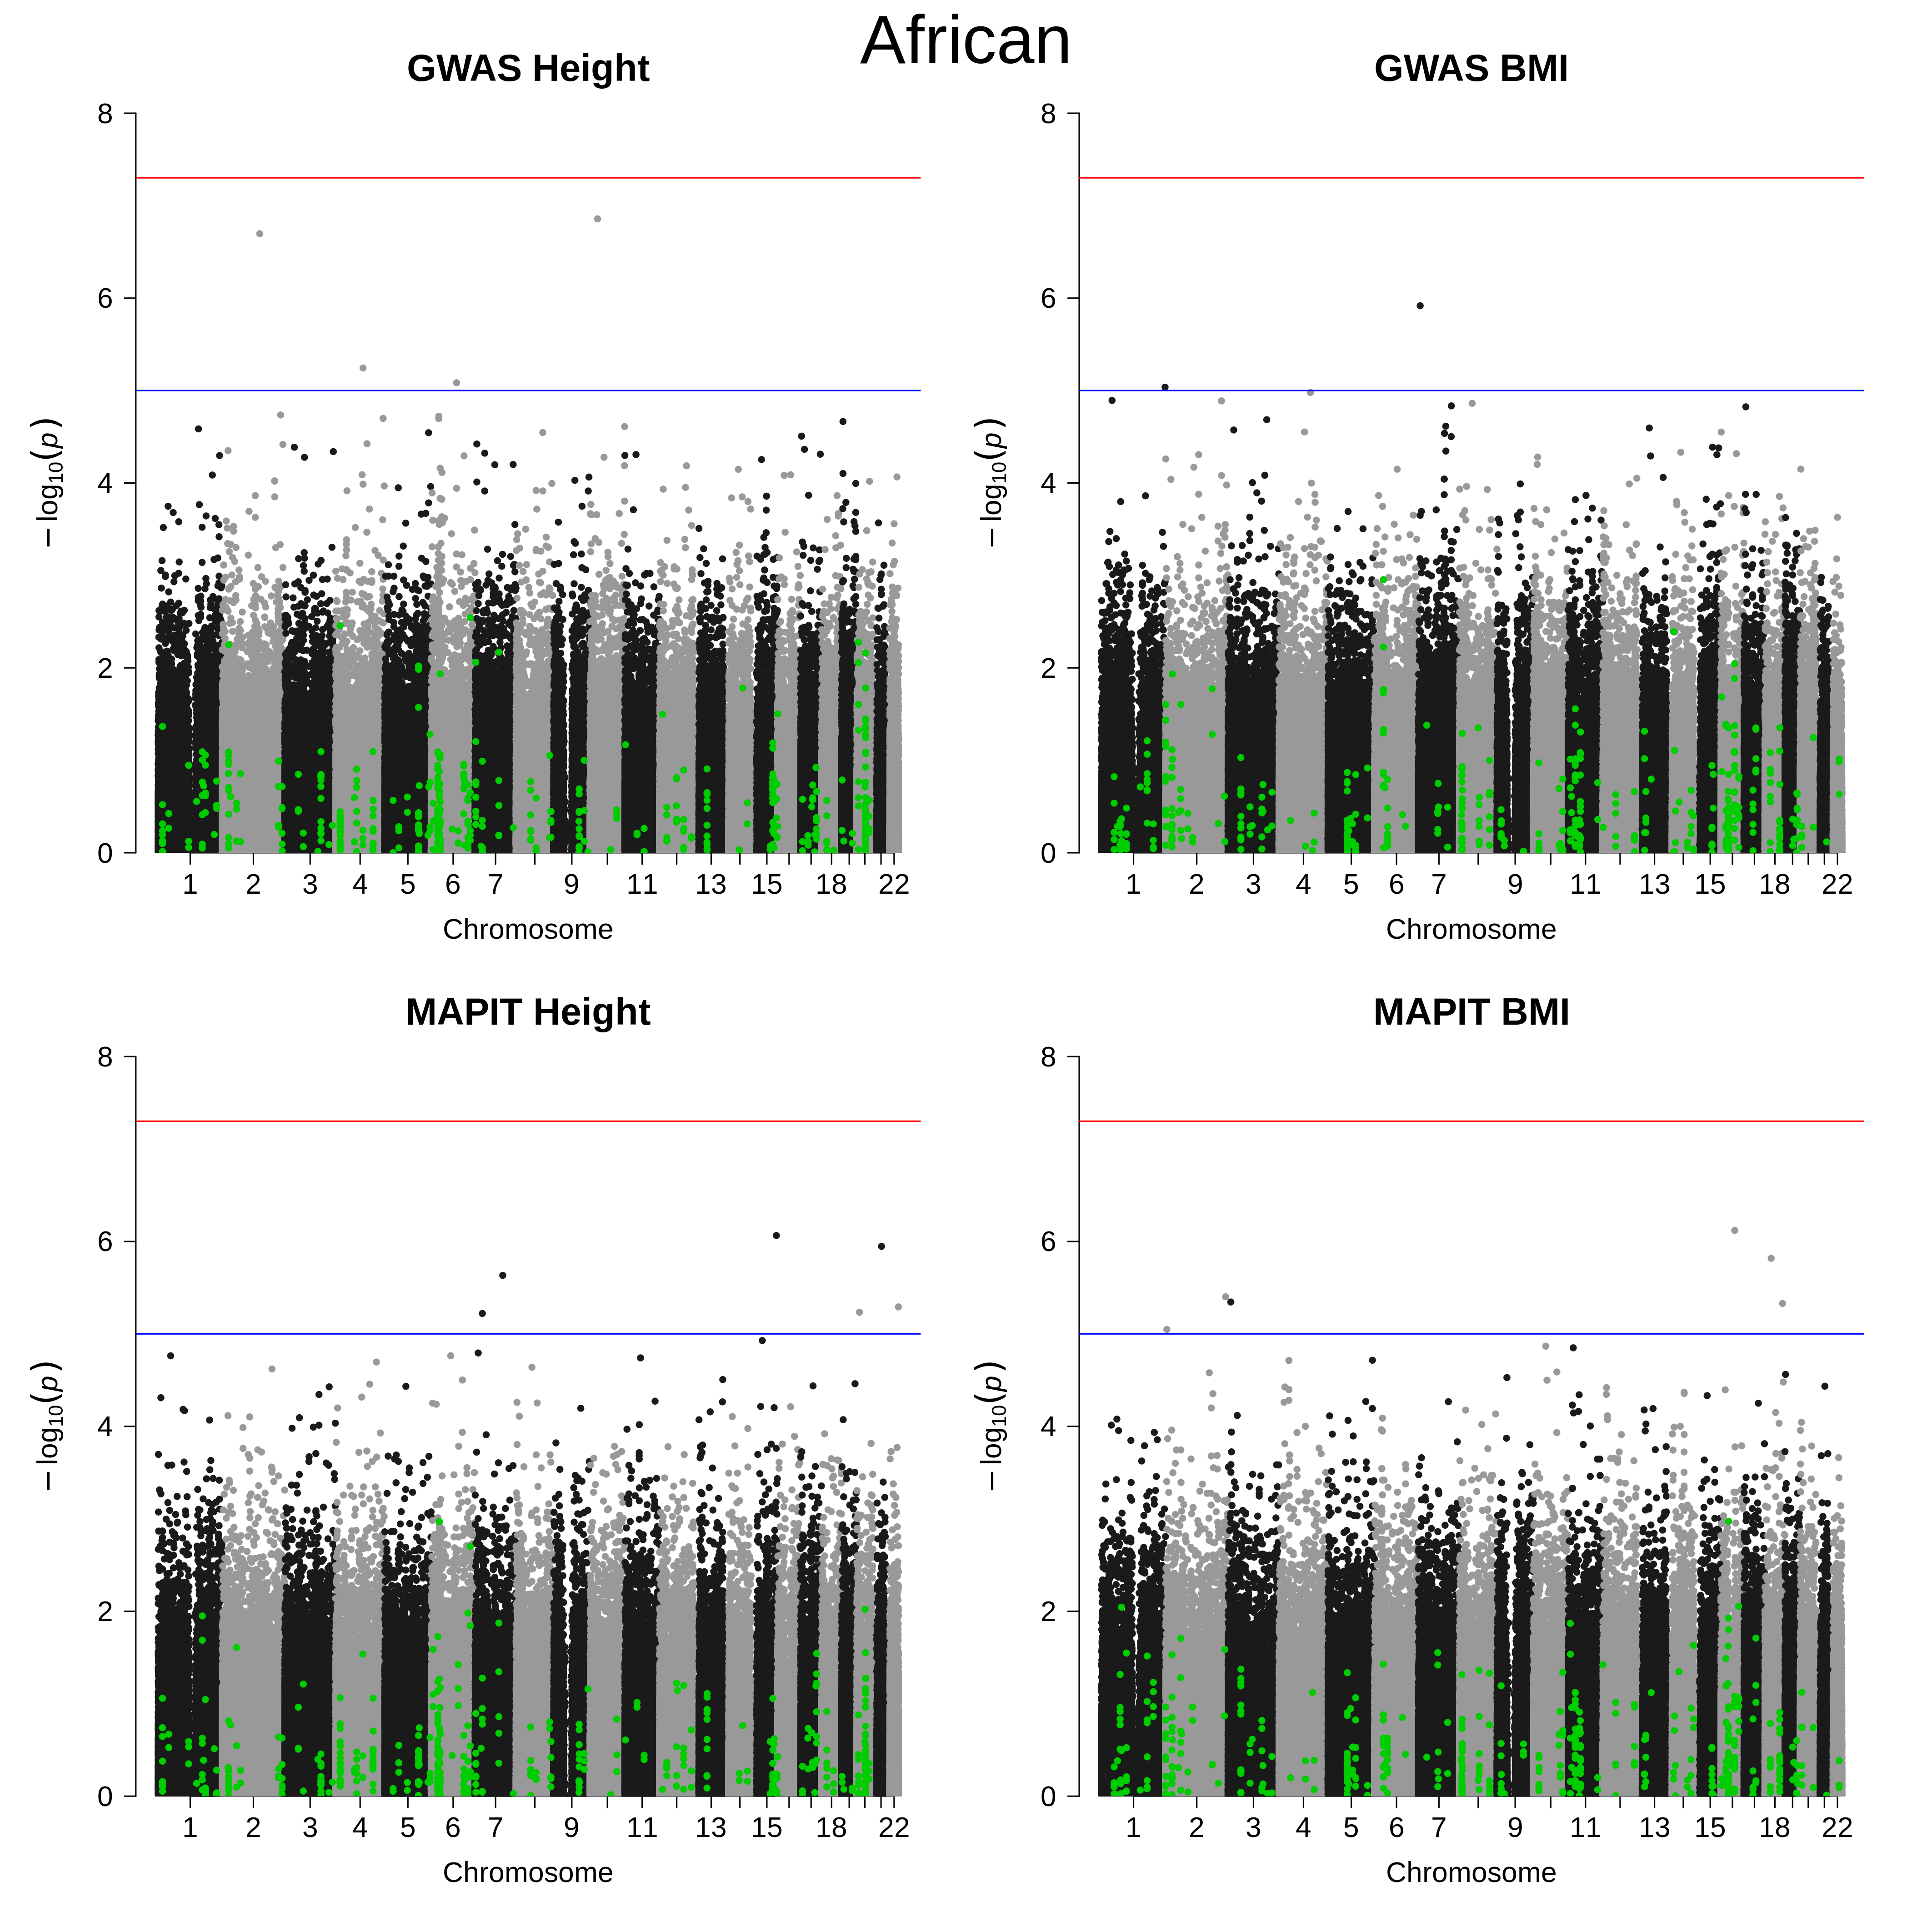
\includegraphics[scale=.35]{Images/Main/InterPath_Main_Figure_MAPITvsGWAS_Manhattan_vs1.png}
\caption[TBD]{\textbf{MAPIT \& GWAS Manhattan Plots}. \textcolor{red}{will be just height, MAPIT on top (D), GWAS on bottom (E), each plot wider. Green dots are the 500 SNPs that have the most significant GIANT/UKB p-values.}}
\label{InterPath-Main-Figure-MAPITvsGWAS-Manhattan}
\end{figure}

%\begin{figure}[htbp]
%\centering
%\includegraphics[scale=.35]{Images/Main/InterPath_Main_Figure_GWAS_Manhattan_vs1.png}
%\caption[TBD]{\textbf{GWAS Manhattan Plot}.}
%\label{InterPath-Main-Figure-GWAS-Manhattan}
%\end{figure}


\begin{align}
    & \textbf{y} = \mu + \textbf{R} + \textbf{G} + \textbf{Q} + \boldsymbol{\epsilon} \\
    \textbf{R} \sim \mathcal{MVN}&(\textbf{0}, \phi^{2}\textbf{K}_R) \quad \textbf{G} \sim \mathcal{MVN}(\textbf{0}, \omega^{2}\textbf{K}_G) \nonumber \\ 
    \textbf{Q} \sim \mathcal{MVN}&(\textbf{0}, \sigma^{2}\textbf{K}_Q) \quad \boldsymbol{\epsilon} \sim \mathcal{MVN}(\textbf{0}, \tau^{2}\textbf{I}) \nonumber 
\end{align}
where now R is a new random effects term that represents our new group of SNPs R, with variance component $\phi$ and GRM $\textbf{K}_R$ based on the SNP set R, and where now $\textbf{K}_Q = \textbf{K}_R \circ \textbf{K}_G$, the Hadamard product between the GRMs constructed from R and G. Similar to the MAPIT model, we construct our 'epistasis' random effect by conducting pairwise multiplication, though now it is between two matrices instead of a vector and a matrix. To see how this changes the additive form of the model, see equation XX in Materials and Methods. We fit this model similarly to before (also see Materials and Methods), and are interested in whether the variance component term $\sigma$ is significantly greater than 0.


Beyond extending our marginal epistasis model, we also expanded the number of UKB data subsets we analyzed given our encouraging results at the single SNP level. Specifically, we added UKB subsets consisting of Chinese, Pakistani, and Irish ancestry, as well as a second random subset of British individuals representing a larger sample size of close to 10,000 individuals. Both the Irish and new, second British subsets represent large sample size subsets to test how our model performs as sample size increases. Lastly, we chose to analyze the KEGG and REACTOME pathways available from the MSigDB \citep{Liberzon2011} due to their coverage of a wide range of biological processes. 




\subsection{GEMMA Analyses}

 the following variance component model:
\begin{equation}\label{InterPath-GEMMA-Equation-Model}
 \textbf{y} = \textbf{G}_1 + \textbf{G}_2 + \boldsymbol{\epsilon}
\end{equation}
where $y$ is a $n \times 1$ vector of phenotypes, $G_1$ is a $n \times n$ genetic relatedness matrix (GRM), constructed using all SNPs genome-wide and representing all first-order interactions, $G_2$ is a $n \times n$ matrix produced from the Hadamard product of $G_1$ against itself ($G_2 = G_1 \circ G_1$), representing all second-order interactions, and $\epsilon$ is a $n \times 1$ vector of normally distributed random effects. In other words, $G_1$ can be thought of as representing all additive effects, and $G_2$ can be thought of as representing all pairwise epistatic effects. To fit this model and estimate $G_2$, we used GEMMA \citep{Zhou2012} and its REML AI algorithm for estimating variance components.

GEMMA/GridLMM analyses were conducted using...







prev abstract

Genome-wide association (GWA) studies have identified thousands of significant genetic associations in humans across a number of complex traits. However, the vast majority of these studies use datasets of predominantly European ancestry \citep{Popejoy2016}. It has generally been thought that complex trait genetic architecture should be transferable across populations of different ancestries, but recent work has shown a number of differences in trait architecture across human ancestries, including heterogeneity in both the identified causal variants and estimated effect sizes 
\citep{Martin2017,Wojcik2019}. Here, we report further evidence that complex trait genetic architecture is fundamentally different among human ancestries by jointly leveraging pathway and epistasis analysis.

Under the assumption that a given complex trait may have differential polygenic architectures across human ancestries, we hypothesize that human populations may also be enriched for differences in epistatic effects. However, since polygenic traits tend to have smaller GWA effect sizes, combining variants via pathway analysis may allow us to better reveal these \red{epistatic?} signals. To accomplish this, we extend the concept of identifying marginal epistasis, moving from testing single variants \citep{Crawford2017} to testing groups of variants for nonlinear association with a trait of interest.

We apply our new method to multiple ancestries present in the UK Biobank \citep{Sudlow2015} and explore multiple pathway-related interaction models. Using morphometric traits we find evidence for genome-wide epistasis in African and other non-European populations. We also find evidence that these trends exists on the SNP and gene levels as well. Results also indicate this may be due to increased heterozygosity in non-European populations. This suggests that non-European populations may be well-suited for identifying non-additive effects in human complex trait architecture; this also suggests further evidence that European populations -- predominantly used for epistasis studies -- may indeed be limited and inaccurate proxies for all human ancestries in complex trait research.

\fi

\end{document}
